\documentclass{article}

\title{Geonomics: A Python package for building agent-based, spatially explicit, and arbitrarily complex landscape-genomic simulations}
\author{Drew Hart}
%\date{January 18, 2019}

%%%%%%%%%%%%%%%%%%%%%%%%%%%%%%%%%%%%%%%%%%%%%%%%%%%%%%%%%%%%%%
% TODO:

% 1] update images

% 2] improve captions

% 3] finish runtime analysis and add that section

% 4] add conclusion

% 5] add citations

% 5] perhaps think through the meaning/implications of the details of the Yosemite example soome more,
% perhaps change some parameters (e.g.\ emulate some specific species; treat each timestep as a year
% and simulate just 100 years and a realistic amount of temperature change
% during that time; parameterize the fitness cost from field data?)

% 6] fix the means by which the Yosemite raster is read in and normalized and used for a 
% Landscape Layer, a K raster, etc; change all of these to raster files that are
% pointed to in the params file and read in from file by Geonomics (as explained in the
% text below

% 7] add better flow diagram

% 8] consider adding diagram of the data structures

%%%%%%%%%%%%%%%%%%%%%%%%%%%%%%%%%%%%%%%%%%%%%%%%%%%%%%%%%%%%%%

% load packages
\usepackage{graphicx} % to include graphics
\usepackage{url}      % to include URLs
\usepackage{fullpage} % use 1-inch margins
\usepackage{amsmath}  % for creating equations
\usepackage[font=footnotesize, labelfont=bf]{caption}  % create figure captions
\usepackage{hyperref}
\usepackage[all]{hypcap} %for going to the top of an image when a figure reference is clicked
\usepackage{cite}     % for bibtex citations

% create typewriter environment
\newenvironment{allintypewriter}{\ttfamily}{\par}


\begin{document}

\maketitle


\section{Abstract}
{\LARGE TO BE COMPLETED}


\section{Intro/Background}
There is ever-growing interest in understanding and even predicting
the genomic evolution of complex study systems on complex and changing landscapes.
Such systems might include one or multiple populations or species that are not
at equilibrium. These species might inhabit complex, multivariate, and even changing landscapes.
And may be undergoing both neutral evolution and natural selection, often on multiple traits
of variable genetic architecture.
Landscape genomics studies the ways in which ecological and evolutionary processes playing
out on real landscapes generate geographical patterns of genomic diversity,
and the field frequently features analysis of data collected from study systems of such
genomic and geospatial complexity.
Study of such systems is crucial for improving our understanding of real-world systems~\cite{pelletier,barrett},
and for better anticipating evolutionary responses to climate change~\cite{bay}
and other sources of environmental change in the Anthropocene.

But the complex genomics of such systems are beyond the reach of analytical
population genetics, and their spatial complexity and multifaceted evolutionary
dynamics make them intractable for coalescent simulation.
This hinders not only our understanding of many empirical systems and our ability to
unambiguously interpret analytical results, but also our
ability to predict those systems' dynamics, and thus to manage them appropriately.
Thus, as is increasingly the case in many fields, forward-time simulation is a 
crucial tool for dissecting the evolutionary dynamics of complex study systems in landscape genomics.
However, the current suite of forward-time genomic simulators, however numerous, is still of limited use for such work.
Most available software is limited, either genomically or geospatially, in the complexity it can model.
Many programs can model systems of considerable genomic complexity
(e.g.\ simuPOP~\cite{peng}, NEMO~\cite{guillaume} and QuantiNemo~\cite{neuenschwander}),
yet incorporate no or only rudimentary spatial components.
Various other programs are designed specifically for landscape-genetic simulations
(e.g. CDPOP~\cite{landguth}, CDmetaPOP~\cite{landguth2}, SimAdapt~\cite{rebaudo}),
but are limited in their genomic complexity.
For instance, many programs are incapable of modeling simultaneous selection on numerous multigenic traits.
To our knowledge, SLiM~\cite{messer,haller}is the only package currently capable of simulating scenarios
that are both as genomically and as geospatially complex as those for which Geonomics is designed~\cite{popgen_models}.
(Indeed, the generalizability and complexity of which SLiM is capable far exceeds that of Geonomics.)

We developed Geonomics to provide a scriptable framework for building
complex landscape-genomic simulations with minimal effort.
Geonomics models are parameterized by way of an informatively annotated parameters file
that provides the user a straightforward means of building models of arbitrary complexity yet offers
reasonable default settings and/or `off switches' for model components that are not the focus the user's interest.
The complex landscape-genomic models for which Geonomics is designed would require a considerable amount
of work to script in SLiM's Eidos framework (see examples of spatialized selection in SLiM 2's recipe book;
e.g.\ section 14.11, page 288;~\cite{slim_manual}), but can be built in Geonomics with as little as three lines of code.
For example, a Geonomics user could build a model of evolution with natural selection
on multiple multigenic traits, on a multivariate landscape undergoing spatially inhomogeneous
environmental change for certain landscape layers, in a species moving realistically across that landscape,
and then run this model an arbitrary number of times, collecting data at various points during each
run --- all of this by doing nothing more than templating a parameters file, making alterations,
loading the file, and running the resulting model object.

What's more, Geonomics is written and run entirely in Python, a broad-purpose and popular
programming language that is already familiar to most researchers with exposure to bioinformatics.
This of course makes Geonomics considerably slower than its brethren that are
written in compiled languages such as C++ (e.g. SLiM). 
But run time is not expected to be a major constraint for the sorts of models
for which Geonomics was built (see runtime analyses, below). 
And what Geonomics sacrifices in performance, it gains in flexibility, extensibility, and accessibility.
In fact, the basic user needn't even need to know how to write full Python scripts to 
build a Geonomics model; users can build their own models by recycling and tweaking
a minimal amount of code (available within the documentation and at the Geonomics homepage).
On the other hand, advanced users wishing to code their own extensions or customizations
have broad opportunity to do so, because Geonomics is a Python package that is seamlessly
integrated into the universe of Python functionality.


\section{Model overview}

\subsection{Components}
A Geonomics model consists of two core components: the species and the landscape.

\subsubsection{Species}
A species consists of an arbitrary number of individuals, which do not belong to
discrete populations but instead are distributed in continuous space upon the landscape.
A species is described by a wide variety of demographic and life-history parameters
that determine its behavior in the model (e.g.\ intrinsic growth rate, mate-search radius,
mean number of offspring per mating event, reproductive age and maximum age, and so on;
for a detailed discussion and these and all other model parameters, see the documentation).
Each species can also undergo any number of arbitrarily complex demographic changes during
each model run, including both population-size changes
(which can be exponential, cyclical, stochastic, or custom-defined)
and changes to various demographic and life-history parameters.

Each individual in a species is described by an x,y location, a sex, an age (or stage),
a genome (optionally), and a phenotype for any traits assigned to the species.
(It is worth noting that species are collected into objects called communities,
which for most models will consist only of a single species,
but which provides a framework for the advanced user 
to code inter-species interactions for multi-species models;
this is a functionality that we hope to build into future versions of the software.)

Each individual has a diploid genome consisting of a $L$ diallelic loci.
These loci can be treated as representing either a contiguous haplotype block
or a set of discrete markers, depending on the map of recombination rates assigned to the genome.
(For simplicity's sake, we refer to these loci herein, and in the software generally, as `the genome'.)
Genomes are initially assigned based on a species' genomic architecture---an object containing
parameters describing all simulated loci.
These parameters include the starting allele frequencies and dominance values for all loci,
the inter-locus recombination rates across the genome.
Separate chromosomes can be modeled by providing a list of chromosome lengths,
between which the recombination rate is set to 0.5, ensuring independent assortment.

A genomic architecture can also stipulate any number of mono- or multigenic traits for a species.
Each trait is defined by a set of loci that underpin it, the effect sizes of those loci,
and a selection coefficient (which can be heterogeneous or homogeneous in both space and time).
Mutations, which are of three types: neutral; deleterious, which universally decrease an individual's fitness); 
and trait-affecting, which influence an individual's phenotype, with the resulting fitness effect
determined by the individual's local environment.
All three mutation types are controlled by type-specific mutation rates 
(additional parameters within the genomic architecture, any or all of which can be set to zero).
(To simulate complex, specific genomic architectures, users can feed into Geonomics a
CSV-formatted file defining the architecture locus by locus. For details, see the documentation.)

\subsubsection{Landscape}
Aside from the species, the other core component in a Geonomics model is the landscape.
A landscape is a stack of an arbitrary number of layers (i.e.\ variables),
each represented by a raster of normalized values ($0 \leq value \leq 1$).
Each layer can be programmed to serve as the basis for any of a number of model components:
1.\ the raster of cell-wise carrying-capacities controlling the population density of a species;
2.\ the resistance surface controlling the realistic movemement of individuals and/or 
dispersal of offspring across the landscape;
3.\ the selective force acting on one or more traits  of one or more species.

Each layer of a landscape can be programmed to undergo any number of
arbitrarily complex environmental change events during each model run.
The changes they produce will in turn affect the dynamics
of any species on the landscape for which that layer plays a role in its
population dynamics, movement or dispersal, and/or natural selection.
Each event is defined by the timesteps over which it unfolds, and either the terminal
raster of the event (with intermediate rasters being linearly interpolated) 
or a directory containing the stepwies time-series of rasters pertaining to the event.
The latter option makes it extremely easy to simulate evolution on real-world
rasters undergoing real, non-linear and spatially heterogeneous environmental change.


\subsection{Operations}
A Geonomics model can be parameterized to run for an arbitrary number of runs,
with each run creating a separate subdirectory of output.
At the start of each run, the must be burned in.
This is accomplished by running the model (without the genomic or
selective components) until a series of statistical tests 
(a time-lagged t-test of mean population size;
an augmented Dickey-Fuller test of population size;
{\large STILL NEED TO ADD THE SPATIAL TEST}) determines that each species'
population size and spatial distribution has reached dynamic equilibrium.
Then, if genomes are being used, each individual has a genome randomly drawn
(according to its genomic architecture) and assigned, such that the main phase
of each model run begins in the absence of any population structure.
At this point, the `main' phase of the run can run for any number of timesteps. 
Each timestep is composed of a series of actions, some requisite, some optional
(see Figure~\ref{fig:flow} for details):
\begin{enumerate}
  \item age/stage incrementation (requisite);
  \item movement (optional);
  \item mate-finding and  mating (requisite);
  \item gamete production (optional, because use of genomes is optional);
  \item offspring dispersal (requisite);
  \item mortality (due to the combination of density-dependence [requisite] and natural selection [optional]);
  \item demographic change events (optional);
  \item landscape-change events (optional);
  \item recording of data and statistics (optional). 
\end{enumerate}

Each individual's age/stage increments at each timestep.
A number of parameters can be set so as to modify a model's behavior on the basis of this attribute
(including the minimum age of reproduction and the maximum age of a species).

Movement takes place in continuous space, such that individuals are not arbitrarily restricted to grid cells.
Individuals' distances and directions are drawn separately, then composed into movement vectors.
Distances are Wald-distributed (and the distributional parameters, as with nearly all distributions
used in the model, can be set by the user within a Geonomics parameters file).
Directions can either be drawn from a uniform distribution on the unit circle, resulting in isotropic movement
(the default behavior); or they can be drawn from a `movement surface' --- an array
of uni- or multimodal Von Mises distributions, derived from a landscape layer that serves as a resistance surface.
The latter option is, to our knowledge, a novel approach to simulating movement,
which generates realistic, anisotropic movment across an environment of heterogenous habitat quality.
(For details, see Figures~\ref{fig:move_surf_hists}~and~\ref{fig:move_surf_tracks}).

Mating pairs are chosen from among all pairs of individuals within the species' mate-search radius
(based on eligibility by age and sex, and decided by a Bernoulli draw with probability equal to the species' intrinsic birth rate). 
For each mating pair a number of offspring is chosen (from a Poisson distribution with
lambda equal to the species' mean number of offspring, unless the user fixes the number of offspring lambda).
Each parent produces one gamete for each of its offspring, by recombination
(at the inter-locus rates defined by the species' genomic architecture) and Mendelian segregation.
Offspring individuals are created and then dispersed to a new location
(where, as with movement, the directions of their dispersal vectors can be drawn either isotropically or
anisotropically, the latter using a `dispersal surface').

Mating is followed by mortality. Deaths are drawn binomially, based on 
individual-wise death probabilities, which are calculated as a combination of
a combination of the probability of death by density-dependence (from a spatialized logistic-growth model)
and the probability of death by natural selection (on any number of traits simultaneously). 
This is calculated as:
\begin{equation}
P(d_{i}) = 1 - (1 - P(d_{x,y})) \prod_{p = 1}^{m}\omega_{i,p}
\end{equation}
where $P(d_{x,y})$ is individual $i$'s probability of death by density-dependence
and $\omega_{i,p}$ is individual $i$'s fitness for trait $p$
(and only factors in if natural selection is being used).
The probability of density-dependent death at location $x,y$ is calculated as:
\begin{equation}
\begin{split}
       P(d_{x,y}) = E[N_{d;x,y}]/N_{x,y} = \frac{E[N_{b;x,y}] - \frac{\mathrm{d}N_{x,y}}{\mathrm{d}t}}{N_{x,y}}
\end{split}
\end{equation}
where $E[N_{d;x,y}]$ is the expected number of deaths at the individual's $x,y$ location on the landscape;
$N_{x,y}$ is the population density (expressed as individuals per cell) at the location;
$E[N_{b;x,y}$ is the expected number of births at the location;
and $\frac{\mathrm{d}N_{x,y}}{\mathrm{d}t}$ is the logistic population growth rate at the location.
Individual $i$'s fitness for trait $p$ is calculated as:
\begin{equation}
\omega_{i,p}= 1 - \phi_{p;x,y} {( \mid e_{p;x,y} - z_{i;p} \mid )}^{\gamma_{p}}
\end{equation}
where $\phi_{p;x,y}$ is the selection coefficient on trait $p$ at the
individual's location; $e_{p;x,y}$ is the environmental value
of the layer that serves as the selective force for trait $p$i,
$\gamma_{p}$ defines the curvature of the fitness function for trait $p$,
and $z_{i;p}$ is individual $i$'s phenotype for trait $p$, which is calculated
from the additive effects of the individual's genotypes at all influencing loci
(Geonomics does not model epistasis) as:
\begin{equation}
        z_{i;p} = g_{0} + \sum_{l = 0}^{n} \alpha_{p,l} g_{i,l}
\end{equation}
where $n$ is the number of loci, $\alpha$ is a locus' effect size, $g$ is the
individual's genotype, and $baseline\_genotype$ is 0 for monogenic traits,
0.5 for polygenic traits. 

Geonomics is designed as an object-oriented scripting framework with both basic and advanced use-modes.
The basic mode simply requires users to call a first command to create a template
parameters file (which they must then edit as desired), a second command to create
a model object from that parameters file, and a third command to then run the desired number
of runs for that model (see Figure~\ref{fig:flow}).
The advanced mode allows users to make modifications to the components of their models,
or to collect custom data from their model, by calling additional functions
before a model is run, between the timesteps of a run, or after a run is complete.
This can be done using both built-in Geonomics functions and homespun Python code.
(This is what makes Geonomics so extensible --- because it is a Python package, users can call on
the full spectrum of Python functionality to design custom code that can interact with Geonomics objects.)

Landscape and demographic change events unfold over some portion of the total time of a run.
The changes are made incrementally, with each incremental change being made 
during each of the timesteps in the series of timesteps defined \emph{a priori} by the user (in the parameters file).
Likewise, statistics are calculated and data are collected
at each of the set of timesteps defined \emph{a prior} by the user.


\section{Validations tests}

\section{Validations tests OLD}
We have run a series of tests to statistically and heuristically validate
the full range of functionality available in Geonomics.
In this section, we briefly review the reasoning and parameterization for each test,
then present the results.
(We discuss only parameters of key importance to each scenario.
Other parameters are set to reasonable values, or left at defaults.
For full details, see the parameters file for a given test.)

All results are as expected, demonstrating a robust ability to reproduce 
population-genetic and population-genomic findings.
Some results show minor deviations from theory.
These artefacts are primarily a resulting of using a simulation framework
designed for complex, spatially explicit models 
to approximate much simpler and, in some cases, aspatial or spatially implicit models.
They artefacts are discussed where applicable.
(The code for all tests is available in the `./tests/validation' directory of the package.)

\subsection{Wright-Fisher test: genetic drift}
The Wright-Fisher model of genetic drift models a fixed-size haploid population that
turns over completely at each timestep (i.e.\ generation).
The population can have any number of independent, biallelic genetic loci.
For each locus, each generation’s allele
frequency is chosen as a binomial random variable, with the number of trials equal to
the population size and the probability of success (i.e.\ of drawing the ‘1’ allele)
equal to the previous generation’s ‘1’-allele frequency.
The mean persistence time for an allele 
(i.e.\ the expected number of generations for which a locus remains segregating) 
is:
\begin{equation}
\bar{t}(p) = -4N[(1 - p)ln(1 - p) + pln(p)]
\label{eqxn:mean_persist_t}
\end{equation}
where $2N$ is the number of alleles in the population (such that $N$ can
represent the diploid population size) and $p$ is the frequency of either allele
at the locus~\cite{wright,fisher,hartl}.

Clearly, the Wright-Fisher model is much simpler than the sorts of models for which
Geonomics is designed (as are all of the following validations tests)---it is aspatial,
panmictic, features fixed population sizes, models only neutral loci, and so forth. 
Thus, we parameterized Geonomics so as to approximate the model as closely as possible.
To emulate aspatiality and panmixia, we used a population on a homogeneous landscape,
with isotropic movement, and with movement and dispersal distributions
and a mating radius that broadly encompass the diagonal width of the landscape.
To enforce complete generational turnover, we set the
maximum age parameter to 1 timestep. While Geonomics does not maintain constant population
size, we maintained the carrying-capacity raster at a constant, uniform value, thus
maintaining a stationary mean population size. We simulated 100, independent neutral
loci (by setting all interlocus recombination rates to 0.5), with starting '1'-allele
frequencies of 0.5 (although the actual starting frequencies vary slightly around
this value because of sampling error when all individuals' genotypes are drawn binomially).

We ran the Wright-Fisher approximation test for three values of the
carrying-capacity raster (i.e.\ three values of `K\_factor'), hence for three mean
population sizes. For each mean population size (calculated as the harmonic mean,
to account for stochastic fluctations around the carrying capacity), we compared
mean persistence time to that
expected by theory, according to equation~\ref{eqxn:mean_persist_t} in the previous paragraph. As can be
seen in Figures~\ref{fig:wf_trajs} and~\ref{fig:wf_persist_vs_popsize}, the results are a close match to theory.


\subsection{Bottleneck test: population dynamics}
Because drift is a stronger evolutionary force in smaller populations,
drift accelerates in shrinking populations. 
If a population undergoes a bottleneck event, the overall effect of drift on the population
during that time is expected to be larger than a constant-size population of equivalent
starting size would experience during that time. 
Thus, mean fixation time should decrease in a bottlenecked population
relative to a constant-size comparison population.

As with the Wright-Fisher model, we used a homogeneous landscape with broad distributions
for movement and dispersal and with a mating radius that encompasses the full landscape
to emulate aspatiality and panmixia. To simulate a bottleneck event,
we created a custom change event in which the population's carrying-capacity raster
is reduced to 30\% of its initial value for 50 timesteps (from the 200th to 250th),
then returned to its initial value for the remainder of the simulation
(through the 2500th timestep).

Figure~\ref{fig:bottleneck} shows a clear signal of drift acceleration during the bottleneck event.


\subsection{Stepping-stone test: population subdivision and genetic differentiation}
The stepping-stone model, or one-dimensional island model, is a spatially implicit model.
It models a series of subpopulations, arranged along a straight line,
with migration between all neighboring pairs.
As a combined result of divergence by drift and homogenization
by effective migration, subpopulations are expected to reach
a stationary level of genetic differentiation---migration-drift equilibrium. 
Theory provides the expected pairwise genetic differentiation
between a pair of subpopulations at equilibrium as:
\begin{equation}
F_{ST} = \frac{1}{1 + 4Nm}
\end{equation}
where $N$ is the population size and $m$ is the per-generation migration rate,
such that $Nm$ can be interpreted as the per-generation number of migrant
individuals~\cite{hartl}.

To approximate the stepping-stone model, we created a Landscape Layer with a diagonal
of six equally spaced islands (1.0-valued cells) embedded in a `sea' of 0.0-valued cells.
We used this layer as the carrying-capacity raster (Figure~\ref{fig:stepstone_pop_and_Fst_mig_expecs}, left).
We set the mating radius to encompass an individual's current island, but no neighboring islands.
We parameterized dispersal to be very local to parents' midpoints, and
parameterized movement distance to be strongly right-skewed, such that
the long-distance movement events leading to migration are uncommon.
We ran the simulation for 5000 timesteps.

Because Geonomics does not model discrete populations, it does not stipulate
migration rates between discrete locations on the Landscape.
Thus we manually tracked the number of migration events during each timestep,
for all possible directional migration events (i.e.\ for all permutations of island pairs),
then used that data to calculate all mean migration rates.
With those values, we solved equation 6, then compared
the resulting $F_{ST}$ expectations to the observed values
(calculated from the simulated data using two common methods; see Figure~\ref{fig:stepstone_pop_and_Fst_mig_expecs} for details).

Results demonstrate that the model has approached migration-drift equilibrium
(Figure~\ref{fig:stepstone_Fst_by_dist}), and that all island populations were at dynamic equilibria around the
same mean size, as expected by theory (Figure~\ref{fig:stepstone_popsize}). 
Estimated migration rates and $F_{ST}$ values qualitatively match theoretical expectations:
mean migration rate drops off precipitously at greater than one island's distance apart, 
and genetic differentiation increases to approximate saturation.
Values of $F_{ST}$ consistently undershoot the values expected based on estimated
migration rates, however, because subpopulations have yet to approach fixation
at most loci (which is the expectation implied by expected $F_{ST}$ values
close to 1).


\subsection{Contrasting-habitat test: adaptive divergence}
In a population divided between two opposite selective environments, if there is
standing genetic variation for a biallelic locus controlling the trait responding
to those environments, then theory predicts that the two subpopulations will diverge at
that locus as each moves toward its respective adaptive peak.
The rate at which divergence should occur depends on the relative strengths
of two opposing evolutionary forces: natural selection, which causes divergence,
and gene flow from migration, which causes homogenization. 
The rate of allele frequency change
in either subpopulation at timestep t is expressed as:
\begin{equation}
\delta{q} = \frac{-spq[q + h(p - q)]}{1 - sq(2hp + q)} + m_{i}q^{*} - m_{o}q
\end{equation}
where $q$ and $p$ are the frequencies of the deleterious and beneficial alleles
in the subpopulation, $s$ is the selection
coefficient against the homozygous recessive phenotype, $h$ is the degree of dominance
of the recessive allele, $m_{i}$ and $m^{o}$ are the migration rates into and out of
the subpopulation being analyzed, and $q^{*}$ is the frequency of the recessive allele
in the alternative subpopulation~\cite{hartl}.

This model, much like the stepping-stone model, is spatially implicit.
To approximate this, we created a landscape with two layers.
The first was divided into two equal-sized halves, one valued at 0.0, the other at 1.0;
this layer was used as the layer driving natural selection.
The second was valued uniformly at 1.0; this was used as the carrying-capacity raster
(thus setting uniform population density across the Landscape and determining,
in sum, the overall carrying capacity of the landscape).
We created one monogenic trait whose position was randomly chosen within a 
genomic architecture of 100 independent (i.e.\ unlinked) loci.
We ran the model for 1000 timesteps for each of three values of the parameter phi
(identical to \emph{s} in equation 7): 0.1, 0.05, and 0.01.
Given that Geonomics does not employ express migration rates,
we tracked the number of migration events (betwen the two contrasting halves of the first layer)
during each timestep, then used that data to solve equation 7.

Results depict clear local adaptation to each of the two halves of the landscape,
with opposite-phenotype bleedover and heterozygote births occuring along
the border between the two habitats (Figure~\ref{fig:div} right).
Allele trajectories in each half of the environment follow qualitatively 
the increasing and saturating trajectories expected by theory,
but reach consistently more extreme allele frequencies than expected (Figure~\ref{fig:div}, left).


\subsection{Cline test: local adaptation}
In a clinal model, a population adapts locally across an environmental gradient,
which is characterized by the extremes of its environmental values and its steepness
(i.e.\ the instantaneous rate of environmental change along it).
Local adaptation across this gradient will generate a cline,
i.e.\ a geographic gradient in allele frequency
(though natural selection is not the only way a cline could be produced).
The clinal pattern is only expected for loci that underlie the trait underoing
selection along the cline (and loci in linkage).
Unlinked loci have no long-term clinal expectation
(though they could initially be swept along with the selective locus adaptation,
and any number could continue to show spurious concordant clinal variation).
To detect clinally adapted loci, we can fit cline curves to the allele-frequency
variation across the environmental gradient for all loci,
with the expectation that the clines fit to adaptive loci will mirror the gradient.
Numerous equations have been used to fit clines, but one of the most common
is the sigmoidal \emph{tanh} function:
\begin{equation}
p_{x} = \frac{1}{2}(1 + \tanh[\frac{2(x - c)}{w}])
\end{equation}
where $p$ is the frequency of the reference allele at position $x$ along the cline,
$c$ is the centerpoint of the cline (such that $p_{x=c} = 0.5$), and $w$ is the 
`width', which is defined as $w = \frac{1}{slope}$ at centerpoint $c$~\cite{porter}. 

To implement the cline model in Geonomics, we created a landscape with two layers.
The first layer was an environmental layer---a symmetrical, non-linear gradient
between 0-valued and 1-valued halves (see raster in both halves of Figure~\ref{fig:cline}).
The second was a uniformly valued habitat-quality layer, used to set a uniform
population density and thus determine the global carrying capacity.
We created a monogenic trait whose locus was randomly placed within a
genomic architecture of 100 independent loci.
The trait had a \emph{phi} (i.e.\ \emph{s}) of 0.01,
with the gradient layer serving as its selective force.

We ran the cline model for 2500 timesteps, then used a numerical optimization function
(in Python's \texttt{scipy} package~\cite{scipy}) to fit \emph{tanh} clines to all loci.
We plotted all fitted clines on top of the first landscape layer,
with the cline for the one selective locus highlighted.
The selective locus consistently and clearly stands out as the only locus with a cline
matching the expectation (i.e.\ mirroring the environmental gradient; Figure~\ref{fig:cline}, left),
and results show an obviously locally adapted population, with a zone of hybridization
and phenotypic spillover surrounding the cline's center (Figure~\ref{fig:cline}, right).
Furthermore, for a family of regression models of environmental value
on genotype for all loci, after Bonferroni correction for multiple testing,
the selective locus is consistently significant and the most significant 
(though other loci produce false-positive results, albeit with considerably larger p-values).
INCLUDE AND SHOW THESE REGRESSION RESULTS?


\subsection{Selective sweep test: genetic hitchhiking}
Genomic context and linkage add important complication to models of molecular evolution.
The most basic model of selection with linkage is that of the selective sweep:
a beneficial mutation occurs in a population, falling on a random genomic background,
then rises in frequency because of its selective advantage until it becomes fixed,
pulling up the frequency of the surrounding haplotype block in the process.
But as the haplotype block increases in frequency it is nevertheless subject to recombination,
which gradually erodes it symmetrically around the beneficial mutaiton.
Thus the selective-sweep model predicts that once a beneficial mutation occurs
---as long as it is not lost early on by chance---
it and the haplotype block around it will rise in frequency,
the mutation will eventually fix, potentially with some core block around it,
but the rest of the block will erode fade over time.
The haplotype block should be clearly visible in genomic data,
where it will manifest as a genomic region of reduced diversity and heterozygosity,
centered on the mutation.

To implement the selective sweep model in Geonomics, we again created a model
approximating an aspatial, panmicitic population (see Wright-Fisher test for details).
We created a single, monogenic trait with a \emph{phi} (i.e.\ \emph{s}) of 0.15.
The trait's locus was manually set to position 50,
such that it was at the center of the the 101-locus genomic architecture.
We manually set the starting '1'-allele frequency at this locus to 0.0,
but set the trait to selected upon by the landscape's first and only layer
(a uniformly 1-valued raster), such that all individuals began the model
equally ill-fit (i.e.\ with a fitness value of $1 - \phi = 0.85$).
After burning the model in, we iteratively chose a random individual,
introduced a '1'-mutation in their genome at locus 50, ran the model for 50 timesteps,
and checked whether the '1' allele had reached a frequency greater than 0.05 by that time.
We iterated until that check was passed, at which point we declared the mutant allele
`established' and continued to run the model until 2500 timesteps
after the mutant reached fixation.
At three timepoints during that model we calculated and recorded
genome-wide nucleotide diversity using a sliding-window approach.

Geonomics realistically emulated the behavior of a selective sweep.
The adaptive phenotype (the '1'|'1' genotype, plotted as white
on a white environmental background; in Figure~\ref{fig:sweep}, top row)
clearly emerged in a region surrounding the mutation's origin,
then spread rapidly throughout the population.
The population's mean fitness increased quickly from 0.85
(the universal fitness value before the mutation was introduced) to 1.00
(the universal fitness value after the sweep was complete; Figure~\ref{fig:sweep}, bottom row, leftmost plot).
The linkage block around the sweeping locus was clearly visible
as a region of depressed nucleotide diversity, which became more pronounced
as the sweep went to completion, then slowly eroded as a result of recombination
of the mutant haplotype's alleles onto non-mutant backgrounds
(Figure~\ref{fig:sweep}, bottom row, second, third, and fourth plots from the left).


\subsection{PCA test: isolation by resistance}
Many real-world populations inhabit landscapes with complex patterns
of hetereogeneous habitat suitability.
The probability of an individual moving across each part of these landscapes
is a function of that part's habitat.
Ecologists often use resistance surfaces (or their reciprocal, resistance surfaces)
to describe movement across such landscapes.
Geonomics' movement surfaces and dispersal surfaces both model such movement
(for individuals' timestep-to-timestep movement and for the dispersal of new
offspring, respectively).
In a population evolving on such a landscape, gene flow between any two locatons on the
landscape is expected to be an inverse function of the resistance-distance between the locations.
As a result of this, a pattern of isolation by resistance (IBR) is expected to develop:
pairwise genetic distances between different populations, or different regions, should be
positively correlated with pairwise resistance distances.

To test this, we constructed a Geonomics model of a single species evolving neutrally
for 1000 timesteps (i.e.\ 1000 rounds of mating) on a randomly generated complex landscape layer,
with that layer serving as the basis for the species' movement surface.
We ran a genetic Principal Components Analysis (PCA) on the full species' simulated genomes,
both after the burn-in (i.e.\ when genomes had just been randomly drawn and assigned to all individuals)
and after the model had run. For each PCA, we extracted the first three principal components (PCs),
scaled them to $0\leq value\leq$, then used the resulting numerals to determine a the
red, green, and blue (RGB) values for the color of each individual.
We used those colors to color each of the individuals in a plot of the full species (using the \texttt{mod.plot()} command).

The results (in Figure~\ref{fig:PCA}) show a clear lack of spatial structure at the outset; because genomes were randomly drawn and assigned,
the population possessed no spatial structure. But more importantly, the results demonstrate significant
spatial strucutre, which maps onto the movement surface's landscape layer exactly as one would expect.
Neutral evolution with realistic movement across this landscape generated a clear and strong signal of IBR.

\subsection{simultaneous-selection test: selection on multiple traits}
{\large FIGURE OUT WHY THESE RESULTS DON'T LOOK RIGHT}
One of the powerful features of Geonomics is that it can simulate on numerous traits simultaneously,
each trait being selected upon by a distinct, and potentially spatially diferentially distributed selective force.
When a population is undergoing selection of this nature, the evolutionary outcome should be a function of the
genomic architecture of the traits (i.e.\ how many loci underlie them, and whether or not their loci are linked),
and of the correlation of the two traits' selective forces in space.

We simulated two scenarios for 1000 timesteps each. Both scenarios are situated on the same
landscape---a landscape with two distinct and uncorrelated selective-force layers: 
one a symmetric, horizontal environmental gradient from 0 to 1, the other a
an identical but vertical gradient.
In both scenarios, the simulated species has a 20-length genome, with 10 distinct loci underpinning
each of the two traits in the simulation (i.e.\ there is no pleiotropy, hence no overlap
in loci between the two traits). However, all loci are independent in the first scenario (recombination
rate = 0.5), whereas all loci are linked in the second scenario (recombination rate = 0.05).

Theory suggests that local adaptation should proceed successfully in the first scenario, but should be
hindered in the second scenario because of genomic conflict resulting from opposing selection
on closely linked loci.
Heuristically, our results corroborate these expectations, with scenario 1 showing a clear
signal of local adaptation (Figure~\ref{fig:two_trait_unlinked}) whereas scenario 2 shows a much messier and more complicated
spatial distribution of phenotypes for each of the two traits (Figure~\ref{fig:two_trait_linked}).


\section{Example use-case: Polygenic adaptation to climate change in the Yosemite region}
- good for now, but reread and edit anyhow


\section{Example use-case: Polygenic adaptation to climate change in the Yosemite region OLD}

Genomics' use and value is best demonstrated by walking through a worked example.
In this section, we explain a complex evolutionary scenario for which 
simulated data is desirable, explain the steps by which we have simulated the
scenario in Geonomics, and then present the results.
(The source code for this example is available within the
\texttt{./example/yosemite} directory of the Geonomics repository.)

There is growing interest in the evolutionary implications of climate change.
Much of this interest focuses on species that are locally adapted along some
environmental gradient that is expected to shift under climate change.
Such environmental shifts can be non-homogeneous spatially
(e.g.\ cooler regions at higher altitudes appear to be warming more
quickly than warmer, low-altitude regions).
Of particular interest the ability for such species to adapt
to changing conditions rather than simply shifting their ranges
and/or being driven locally extinct.

We simulate an example of such a study system: the adaptive
response of a hypothetical, continuously distributed, locally adapted species
to spatially heterogeneous climate change in the Yosemite region.
To do so, we began by downloading a raster dataset of 30-year
temperature normals for the Yosemite region (from Cal-Adapt; \url{www.caladapt.org}),
cropped it to a 90-cell by 90-cell window surrounding the Yosmite valley,
and saved the cropped file.
We then wrote a couple short Python functions to produce from that raster
the full set of rasters needed for the simulation
(including current and projected future temperatures,
and current and project future habitat suitability).

Temperature is the environmental variable driving natural selection. 
In order to model adaptive responses to change in this variable,
we needed a raster of future temperatures,
to feed into a landscape-change event as the endpoint raster.
We could have downloaded a series of future-projection rasters and loaded
them in as the stepwise changes for the environmental-change event,
because Geonomics is designed to accept a directory of such files.
However, to keep things simple we just processed the 30-year normals raster
with a simple heuristic function.
That function adds to the 30-year normals raster a fixed, region-wide
temperature increase (2 degrees) plus an additional, elevation-dependent fraction
of that increase (where there fraction varies from
0.0 at the hottest cell to 1.0 at the coldest cell).
This function emulates the fact that warming due to climate change is quickest at higher elevations.
We saved the resulting future-temperature raster to a new raster file.

We also needed habitat-suitability rasters for the model.
These must reflect the fact that species tend to find highest-quality habitat,
and thus exist at their highest densities, in the core of their range,
and that edge habitat becomes increasingly marginal. 
Thus we wrote a function that accepts the temperature raster as input and produces from
it a second habitat-suitability raster (where cells with temperature values
between 7 and 11 degrees Celsius are assigned a 1.0 quality value,
and cells outside that range are assigned suitability values that linearly decrease
to 0.0 in the hottest and coldest cells in the raster).
We fed both the 30-year normals raster and the future temperature raster through this function,
thereby generating both current and future habitat-suitability rasters,
which we saved to new raster files.

With these rasters prepared, we then created a Geonomics parameters file.
We needed to parameterize a model with 2 `file'-type Layers
(i.e.\ layers red in from files; see the Geonomics documentation for details),
both of which would undergo landscape-change.
We also needed to model to contain 1 Species,
with movement, a movement-surface, and genomes with 1 trait.
And we needed the model to carry out data-collection.
The Geonomics command we ran to generate a template Geonomics parameters
file with those components was:

\begin{allintypewriter}
>>> gnx.make\_parameters\_file(filepath=`yosemite\_params.py',\\
                               layers=[\{`type': `file', `change': True\},\\
                                       \{`type': `file', `change': True\}],\\
                               species=[\{`movement': True, `movement\_surface': True,\\
                                          `genomes': True, `n\_traits': 1\}],\\
                               data=True)\\
\end{allintypewriter}

After running this command, we opened the resulting, auto-generated parameters
file (\texttt{yosemite\_params.py}) and edited the parameters as needed.
In the Layer `init' and `change' parameters sections we replaced
the placeholder filenames with the names of the four temperature-derived
rasters whose creation is explained above.
We also parameterized the landscape-change events:
both Layers would change from their original rasters to their final
rasters in 20 stepwise changes over 1000 timesteps (i.e.\ 1000 years),
starting on timestep 499 and finishing on timestep 1499.
We stated that the habitat-quality layer would serve as the basis for the movement-surface.
And we parameterized the model to include no mutation.
We stipulated the selection coefficient (\emph{phi}) on the trait (0.05),
and the number of loci underlying it (100 randomly-selected loci).
We left all other parameters at default values.

Finally, we wrote a short script to:
\begin{enumerate}
  \item create a model from the parameters (`mod = gnx.make\_model('./yosemite\_params.py')`);
  \item manually burn in and run the model (using the \texttt{mod.walk} function to run the model
in either `burn' or `main' mode for the desired number of timesteps;
  \item plot the model at various timesteps, using \texttt{mod.plot\_<\_>} functions or manual \texttt{matplotlib} code.
\end{enumerate}

The model generated a clear and realistic pattern of polygenic adaptation to
the elevation-based temperature gradient in the Yosemite region, and that
gradient of local adpatation exhibited a pronounced upslope shift in response to
the period of climate change. These results are visible both heuristically
(from the individuals' phenotypes plotted across the three discrete timesteps' columns
in Figure~\ref{fig:yosemite})
and analytically (from the rasters of neighborhood-meaned phenotype plotted across
Figure~\ref{fig:yosemite}, row 3).


\section{Caveats and considerations}
- runtime analyses (basic), and explicitly point out the key concerns/parameters
that users should think about for runtime and memory usage constraints (including, e.g.,
a layer that serves as basis for movement-surface and that changes a lot)
- need to discuss the weird approach to mutation?


There are two unconventional approximations that Geonomics uses,
in order to make such complex models tractable in Python within a reasonable amount of compute-time.
The first is the approximation used to model recombination along a simulated genome.
Precise modeling of recombination between all loci when each gamete is produced
would require an extremely large number of Bernoulli draws---
roughly $2LbT$, where $2$ represents diploidy, $L$ is the length of the genome,
$b$ is the mean number of births per timestep, and $T$ is the number of timesteps.
So as to avoid generating such a large amount of random numbers throughout a model run,
when a Geonomics model is first created, Geonomics generates and saves
(as binary arrays) a large collection of recombination paths (the exact number of which can
be parameterized by the user).
(A recombination path is a locuswise map along a pair of homologous genomes,
represented as 0 and 1, where a switch between 0 and 1 at each locus is drawn as a Bernoulli
random variable with success equal to the rate of recombination between that locus and the next.)
Then, the paths are repeatedly shuffled and drawn through (think of a deck of cards)
and used to index new gametes out of the genomes of reproducing individuals.
In this way, free and potentially heterogeneous recombination is approximated.
We feel that this is a reasonable approach that balances the needs of the system being modeled
with the constraints of the interpreted language being used for the model,
and that poses no risk of creating systematic artefacts.
However, the user should be aware of two concerns:
1. The total number of recombination paths generated
(which is controlled from the parameters file) determines the precision with which truly 
free recombination at the stipulated genome-wide recombination rates is approximated.
2. The total number of paths also dictates the precision at which close recombinations
rates can be differentiated, because all loci with non-zero recombination rates are forced to
have at least a single recombination rate among the set of recombination paths that are generated
(e.g., the smallest recombination rate that can be modeled when 10000 recombination paths
are used is $1/10000=10\exp^{-4}$, such that a locus with a nominal recombination rate of 
$10\exp^-5$ would be inaccurately modeled as recombiningwith a probability of $10\exp^{-4}$). 
When necessary, Geonomics raises relevant warnings about this at the time that a model is created.

The other approximation of which users should be aware
is that of movement across a heterogeneous resistance layer.
This is implemented by the movement surface and dispersal surface objects
(both of which are identical in structure and function).
Conceptually, a movement or dispersal surface is an $x$x$y$ array of VonMises (i.e circular)
probability distributions. Each distribution pertains to its corresponding landscape cell,
and for an individual located on that cell and about to undergo movement or dispersal
it is used as the distribution from which the individual's direction is drawn.
The distributions can be made either uni- or multimodal (i.e.\ either single VonMises distributions
or VonMises mixture distributions), and they represent the probability of an individual in a given
cell moving in all directions, based on the environmental values in the surrounding cells.
Programmatically, this is implemented using an array of vectors of draws from the distributions,
such that the vectors serve as approxiations of the true distributions (much like unbinned histograms).
Thus, a movement or dispersal surface is structured as an $x$x$y$x$z$ \texttt{numpy} array,
where $x$ and $y$ are the x- and y-dimensions of the landscape and $z$ is the length of the
vectors approximating the true distributions.
This structure is built when a model is first created, and then allows us to simulate realistic
movement across a complex landscape without the need to run neighborhood-querying functions
(which are notoriously costly) during each model run.
However, the accuracy of the approximations of the true distributions is a function of
the length of the approximation vectors.
For complex landscapes, users may wish to ensure the accuracy with which their movement or
dispersal surfaces reflect the true heterogeneity in their resistance layers.
Geonomics provides a number of built-in visualization functions to aid in heuristic checks of this sort.


\section{Getting started}
For those interested in using Geonomics, the simplest way is to install
via \texttt{pip} (a Python package installer),
by calling \texttt{\$ pip install geonomics}.
(Note that Geonomics only uses common, well established Python packages
as required dependencies:
\texttt{Numpy}~\cite{numpy},
\texttt{Matplotlib}~\cite{matplotlib},
\texttt{Pandas}~\cite{pandas},
\texttt{Shapely}~\cite{shapely},
\texttt{Scipy}~\cite{scipy},
\texttt{Scikit-learn}~\cite{scikit-learn},
\texttt{statsmodels}~\cite{statsmodels},
\texttt{PyVCF}~\cite{pyvcf},
and \texttt{Bitarray}~\cite{bitarray}.
The source code is also publicly available on GitHub (\url{URL\_HERE}),
where it is actively maintained and developed.

The documentation is comprehensive (and will continue to expand as new worked examples
are offered and new functionality is added to the package), and is available
online at \url{http://htmlpreview.github.io/?https://github.com/drewhart/geonomics\_docs/blob/master/built/doc.html}.  
The simplest and advanced use cases are explained above (see section
\emph{Design, structure, and function}), as well as in the documentation.
The documentation provides a detailed section explaining the meaning,
default values, and usage for every parameter in a Geonomics parameter file.
Details about the usage of each function are available both in the documentation
and in the docstrings (the latter of which can be accessed by by calling Python's
\texttt{help()} function on a function of interest).


\section{Conclusion}
- very very brief summary of, once again, Geonomics' design-purposed ability
- think it should be very helpful for running simulations of high utility to
  molecular ecology, conservation, etc. 
- should be valuable for theoretical, methodological, empirical, and applied research
- expandibility planned in advance (e.g.\ multi-species models foreseen)


\section{Works Cited}
\bibliographystyle{plain}
\bibliography{articles_etc,pkgs}

\pagebreak
\section{Figures and Captions}

% fig 1
\begin{figure}[h!]
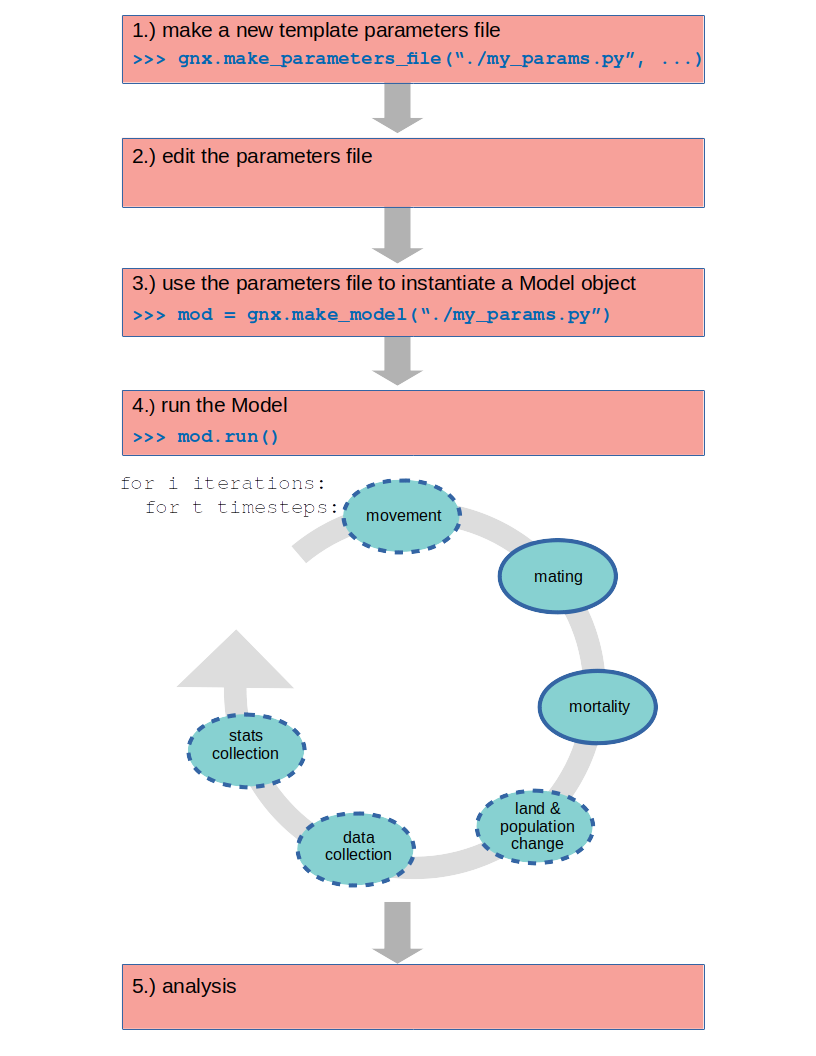
\includegraphics[width=125mm]{./img/flow_diagram.png}
        \caption{Geonomics flow diagram}
        \label{fig:flow}
\end{figure}


% fig 2
\begin{figure}[h!]
\includegraphics[width=225mm]{./img/move_surf_histograms.png}
        \caption{Histograms of the VonMises mixture-distribution approximations in a movement surface, plotted over a small landscape layer on which the surface is based. The taller the bar in a histogram, the higher the probability that an individual located on that histogram's cell will move in a direction within the angular neighborhood of that bar.}
        \label{fig:move_surf_hists}
\end{figure}

% fig 3
\begin{figure}[h!]
\includegraphics[width=225mm]{./img/move_surf_tracks.png}
        \caption{Examples of movement tracks for 25 individuals randomly selected from a species, moving across the movement surface depicted in Figure 2. Each track is 150 steps long, beings at the individuals' starting locations (white dots), and thickens with each increasing timestep. Individudals' preference for higher-suitability regions of the landscape (values with environmental values nearer 1) is evident. Occasional migrations between isolated portions of the landscape can also be seen.}
        \label{fig:move_surf_tracks}
\end{figure}



% fig 4
\begin{figure}[h!]
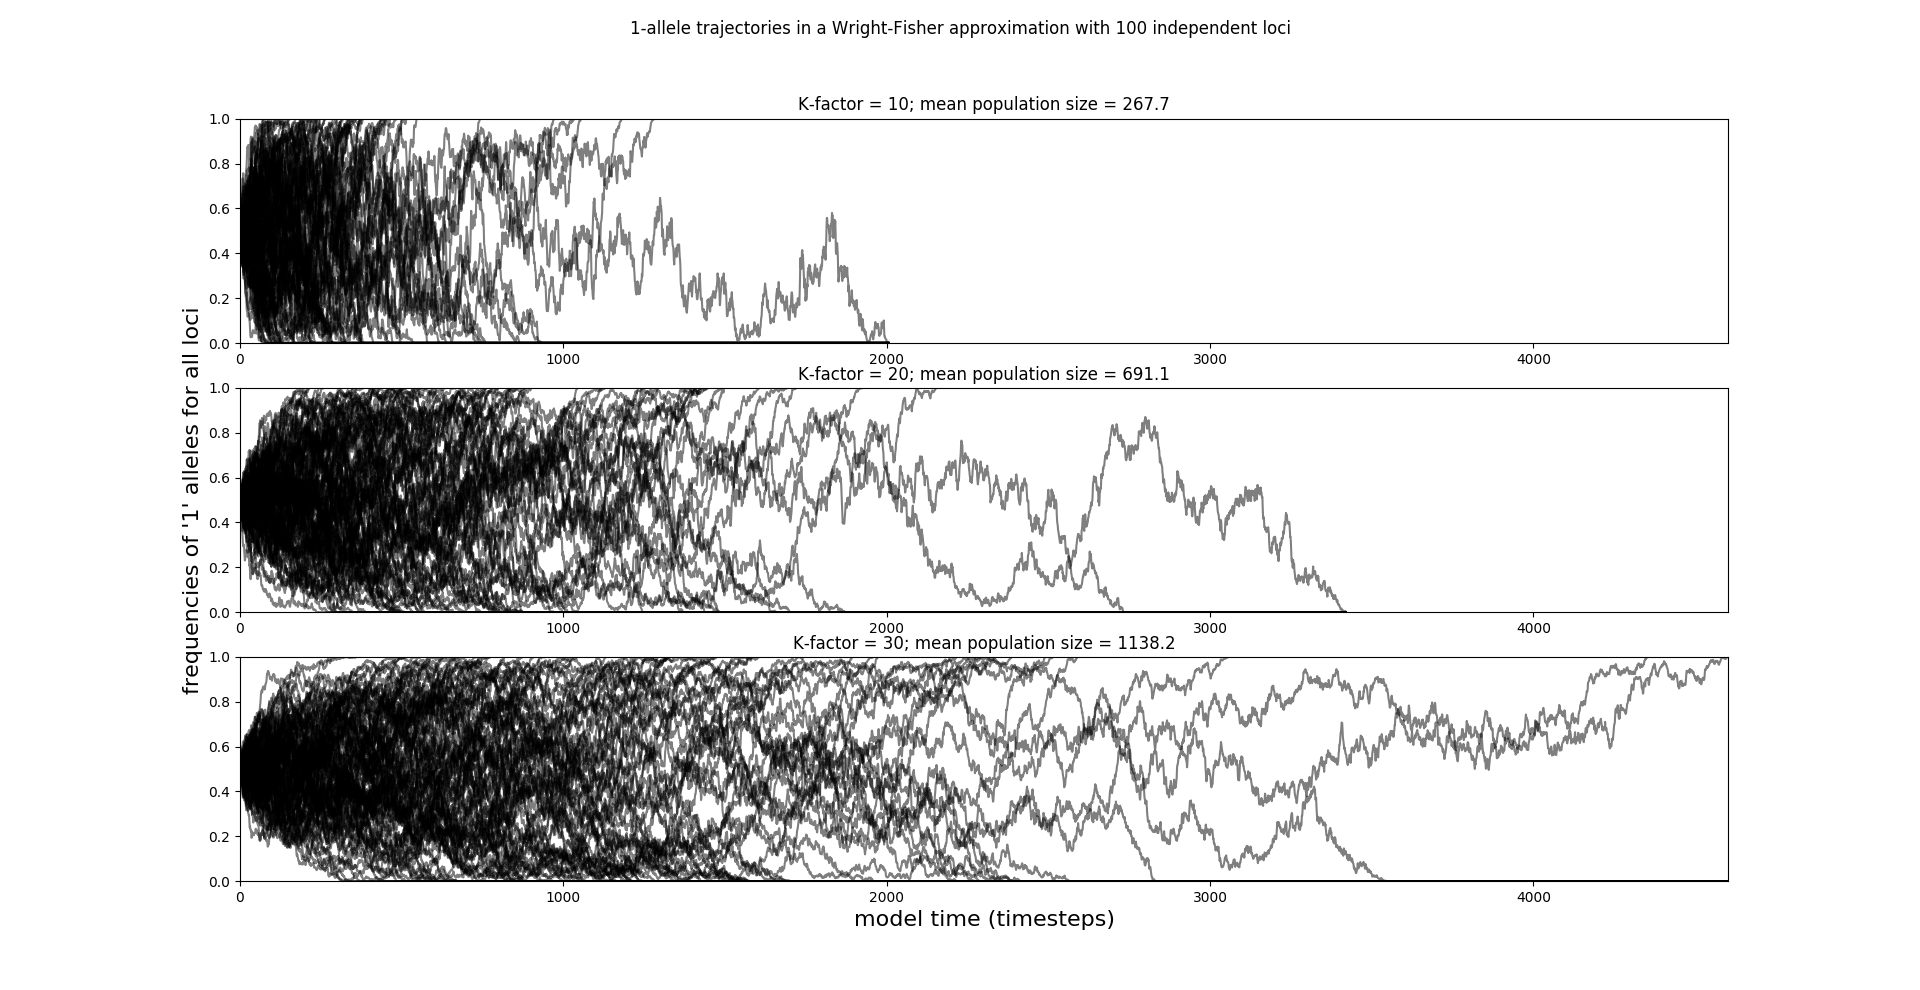
\includegraphics[width=175mm]{./img/validation/wf/allele_trajectories.png}
        \caption{Wright-Fisher test: allele-frequency trajectories; each line shows the trajectory of the '1'-allele for a different locus}
        \label{fig:wf_trajs}
\end{figure}


% fig 5
\begin{figure}[h!]
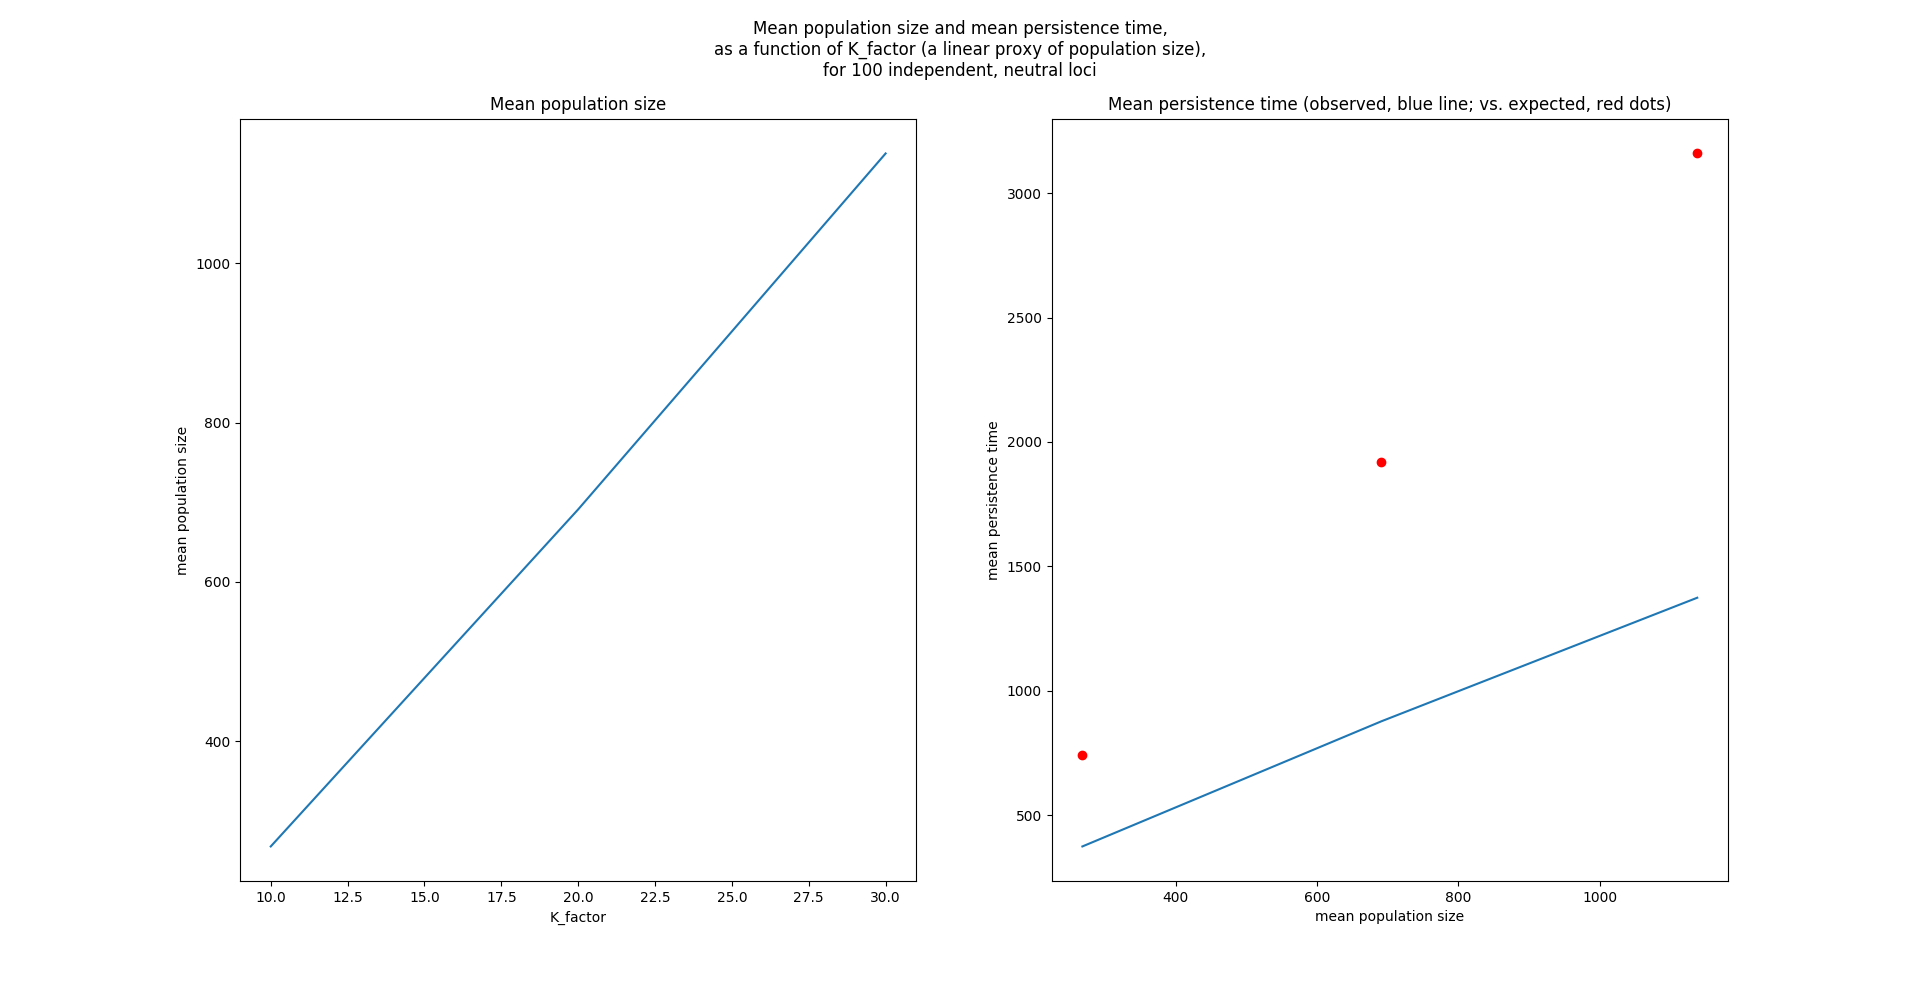
\includegraphics[width=175mm]{./img/validation/wf/pop_size_vs_K_factor_and_mean_persist_t_vs_pop_size.png}
        \caption{Wright-Fisher test: left: mean population size as a function of `K\_factor' (multiplicative factor determining a species' spatialized carrying capacity and thus equilibrium population size; right: mean persistence time for segregating sites as a function of mean population size)}
        \label{fig:wf_persist_vs_popsize}
\end{figure}


% fig 6
\begin{figure}[h!]
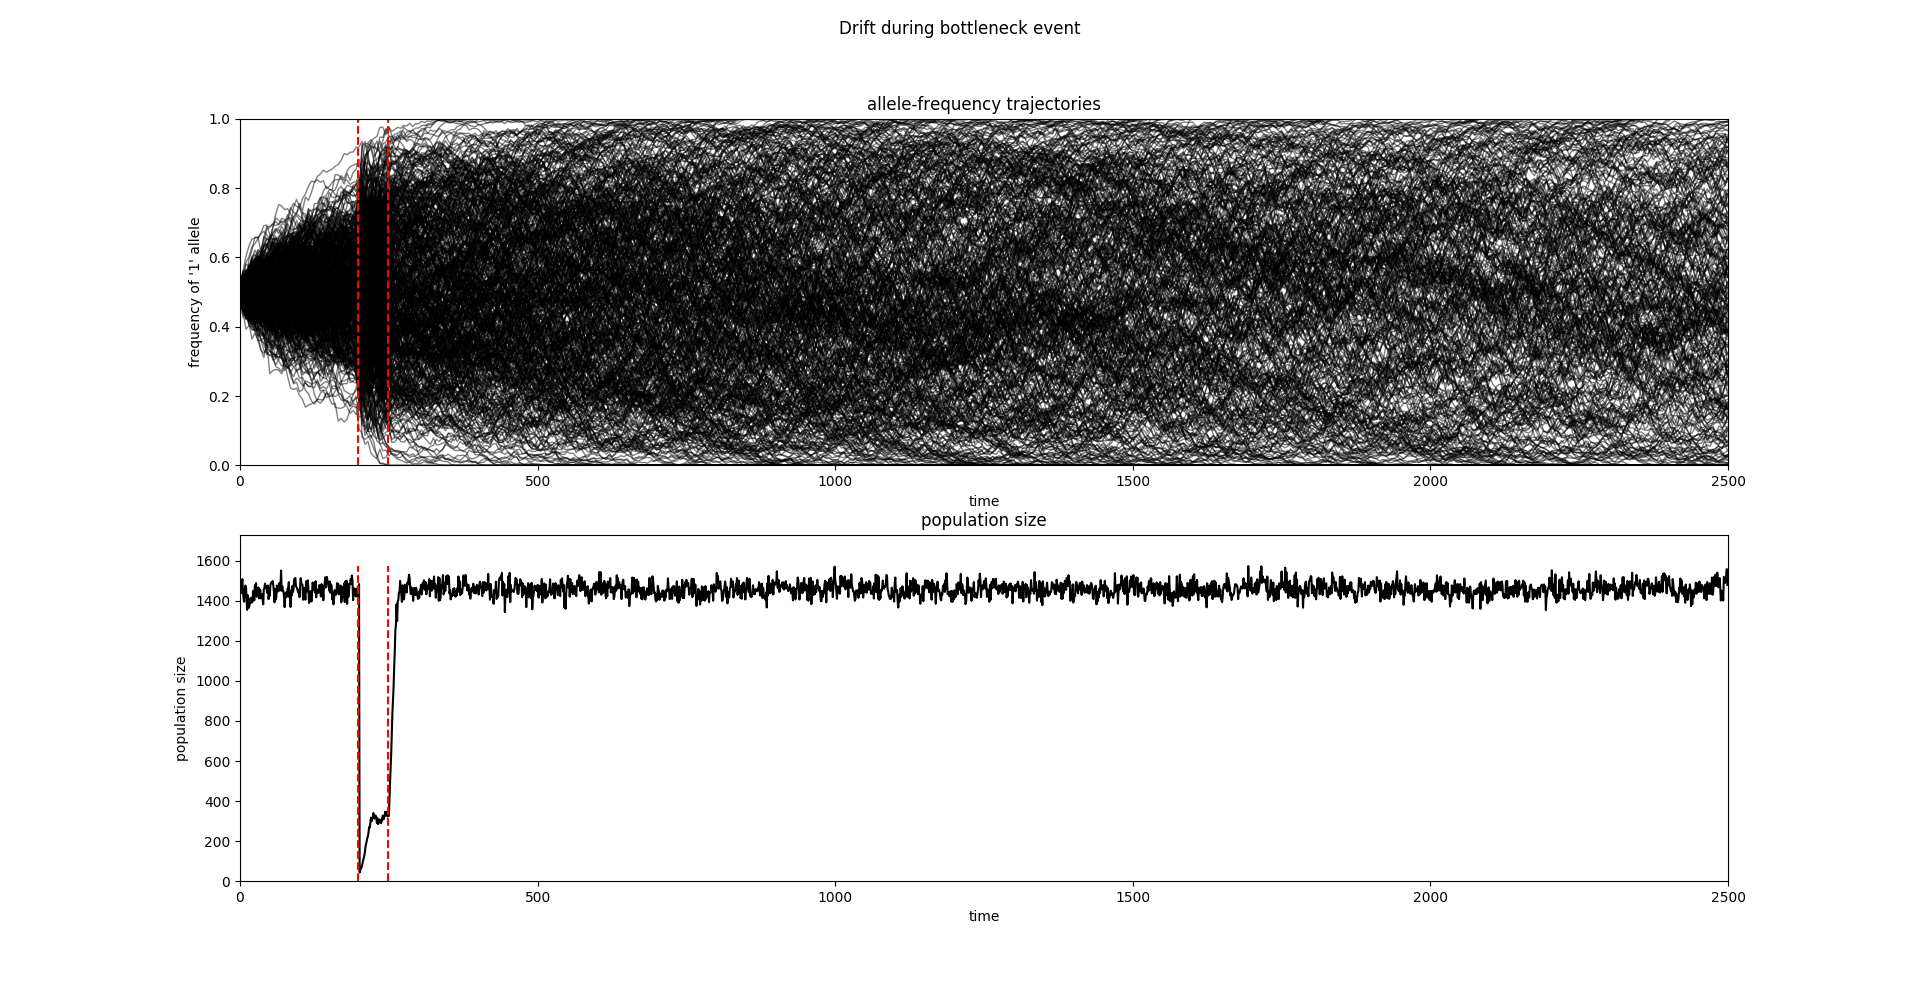
\includegraphics[width=175mm]{./img/validation/bottleneck/alleles_seem_to_take_too_long_to_fix.png}
        \caption{Bottleneck test: 1-allele frequencies (top) and population size (bottom) as a function of time}
        \label{fig:bottleneck}
\end{figure}


% fig 7
\begin{figure}[h!]
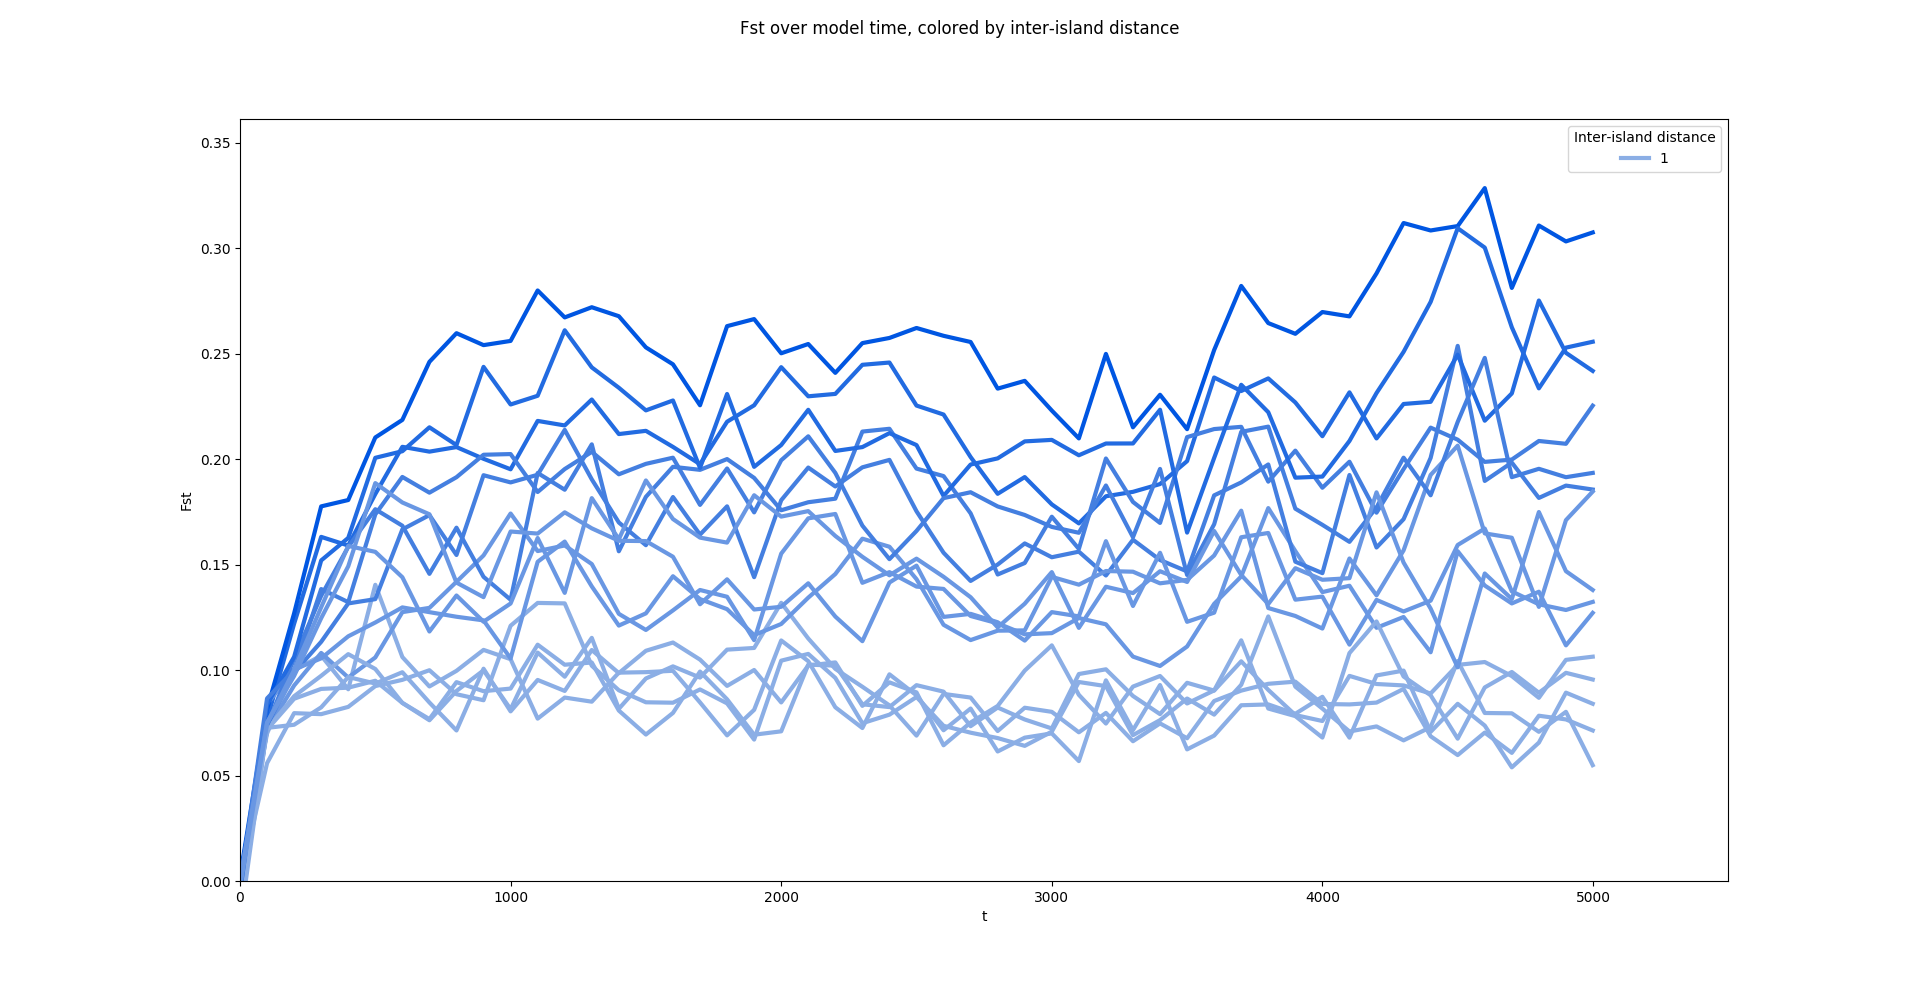
\includegraphics[width=175mm]{./img/validation/stepping_stone/Fst_over_time_vs_interisland_dist.png}
        \caption{Stepping-stone test: $F_{ST}$ as a function of model time, across increasing inter-island distances (gradually darker shades of blue)}
        \label{fig:stepstone_Fst_by_dist}
\end{figure}


% fig 8
\begin{figure}[h!]
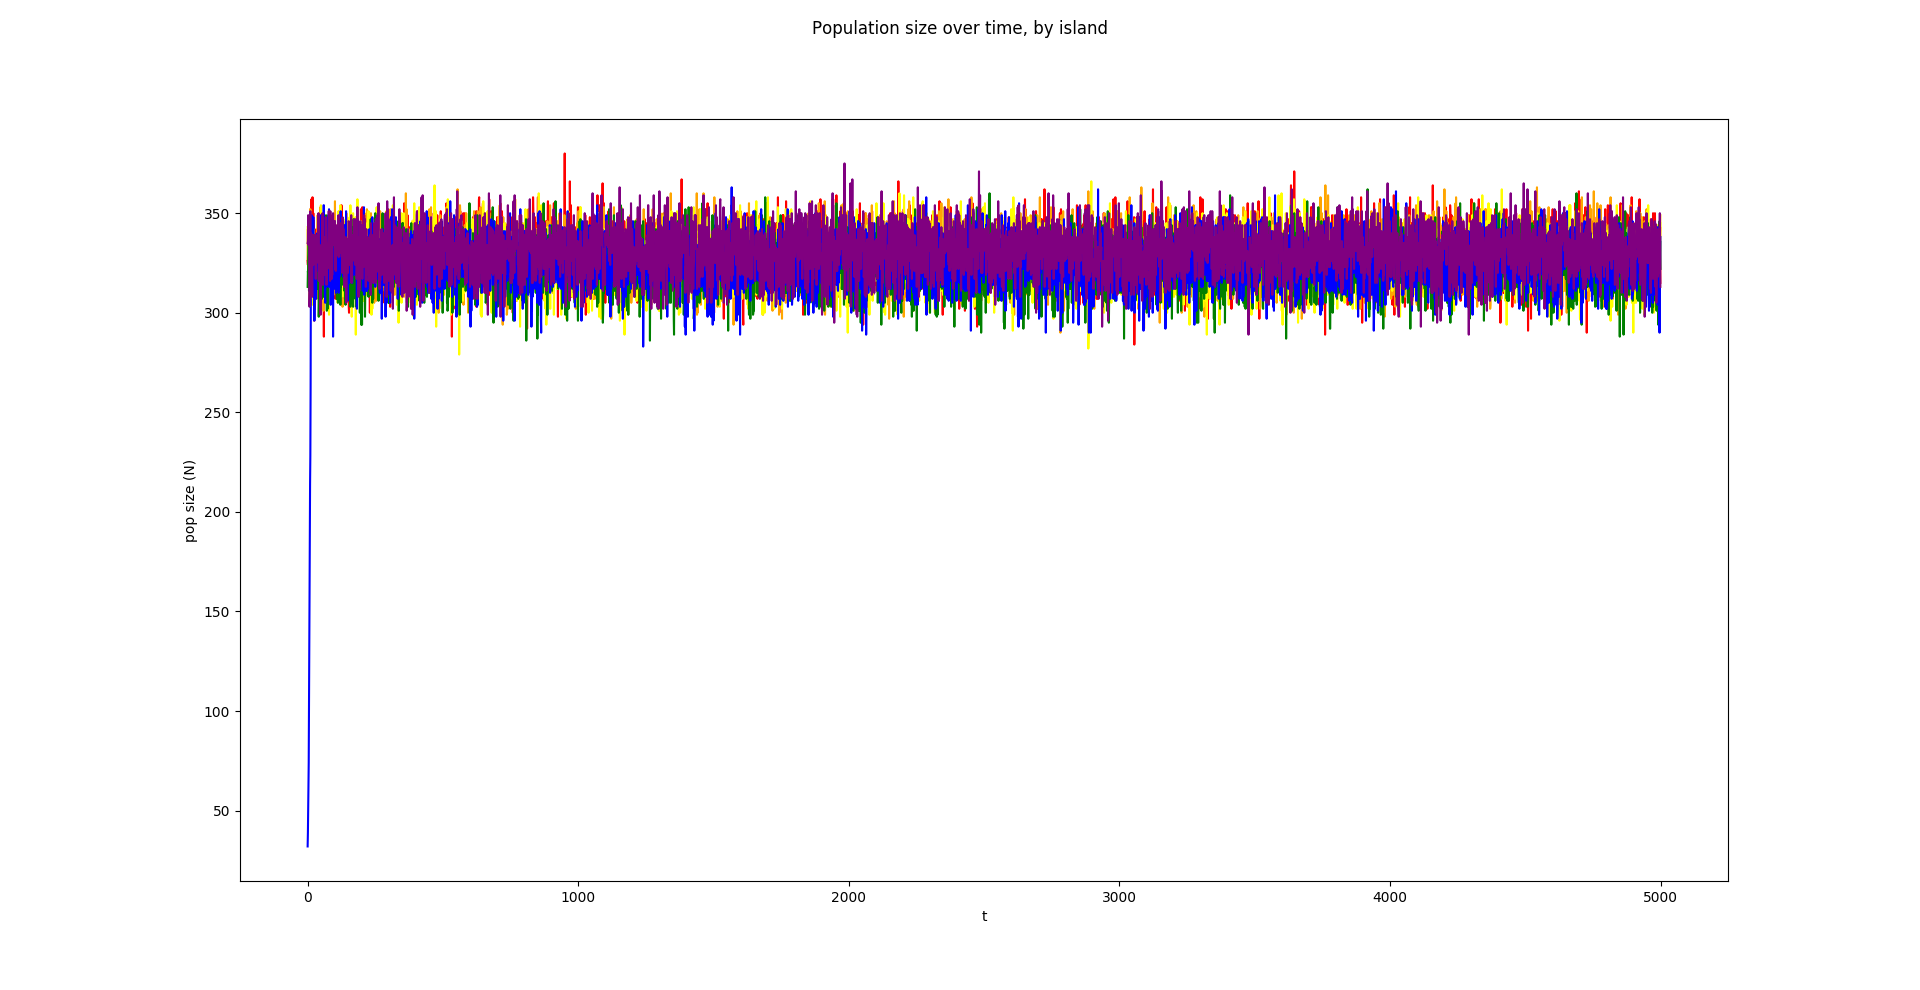
\includegraphics[width=175mm]{./img/validation/stepping_stone/pop_size_over_time.png}
\caption{Stepping-stone test: Population size as a function of time, for all 6 islands' populations}
        \label{fig:stepstone_popsize}
\end{figure}


% fig 9
\begin{figure}[h!]
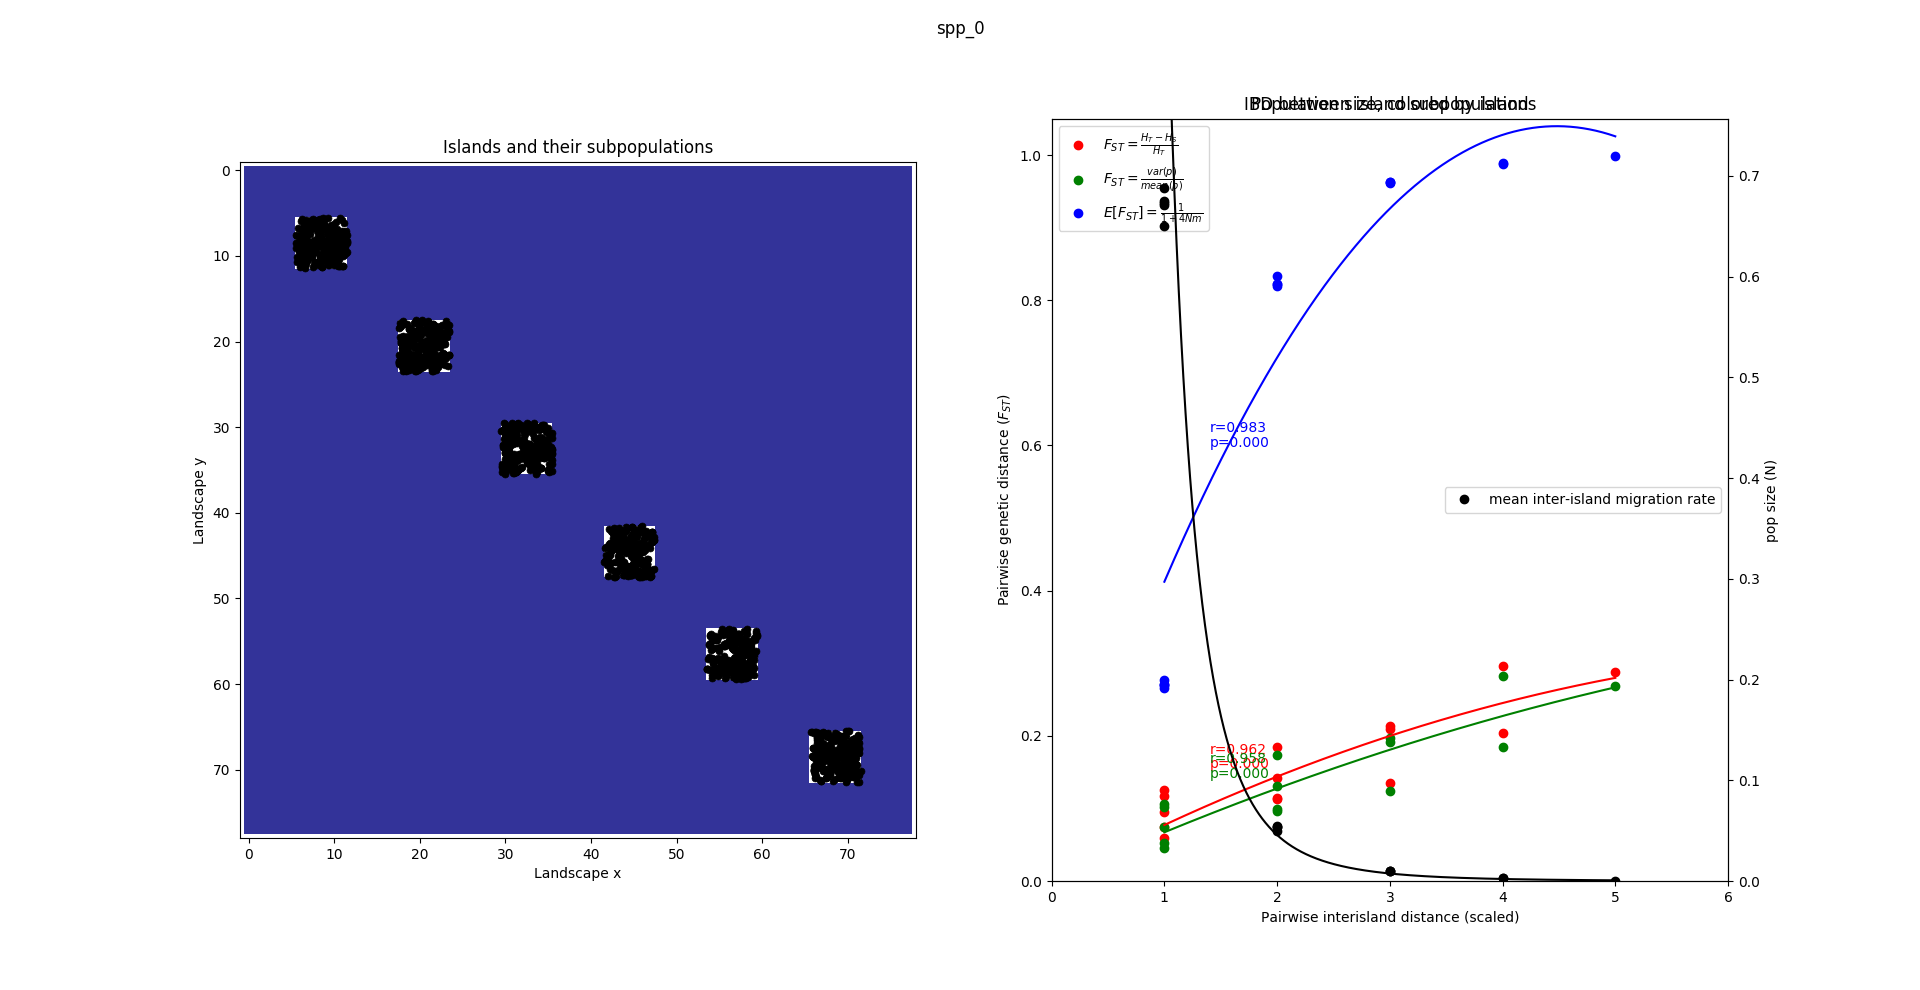
\includegraphics[width=175mm]{./img/validation/stepping_stone/pop_plot_and_Fst_and_mig_rate_plot.png}
        \caption{Stepping-stone test: left: Map of all 6 islands' populations at the end of the simulation; right: pairwise $F_{ST}$ (left y-axis; calculated by 2 different formulae) and inter-island migration rate (right y-axis) as a function of inter-island distance; $R^{2}$ values and p-values result from quadratic regressions of $F_{ST}$ values on inter-island distance and log-log regression of mean migration rate on inter-island distance}
        \label{fig:stepstone_pop_and_Fst_mig_expecs}
\end{figure}


% fig 10
\begin{figure}[h!]
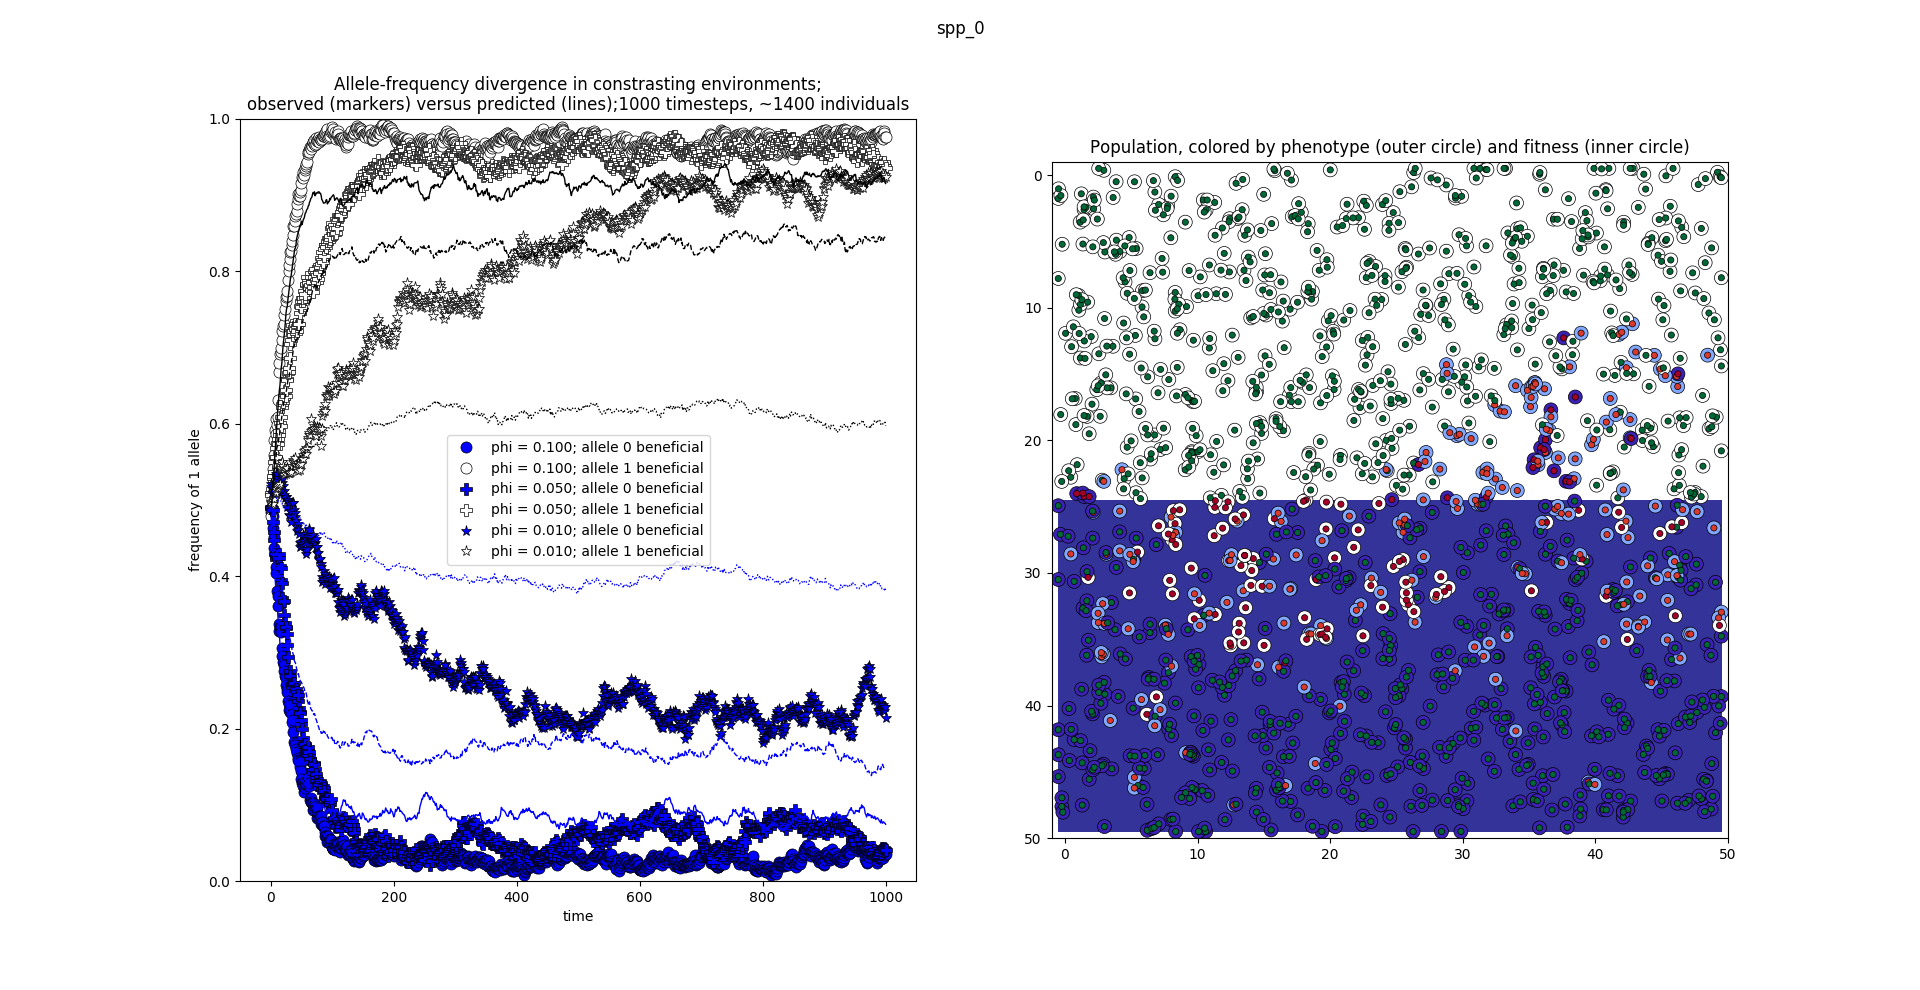
\includegraphics[width=175mm]{./img/validation/divergence/divergence_test_ca1400_individuals_1000_timesteps.png}
        \caption{Contrasting-habitat test: left: Observed (markers) versus predicted (lines) allele-frequency trajectories for two contrasting habitats (blue = 0.0-valued; white = 1.0-valued), across three selection coefficients ($\phi$ = 0.01: stars; 0.05: crosses; 0.10: circles); right: map of the population after spatially divergent selection at $\phi$ = 0.10, with individuals, colored by phenotype (outer circles) and fitness (inner circles), plotted on top of the selective landscape layer (horizontally divided into white and blue halves)}
        \label{fig:div}
\end{figure}


% fig 11
\begin{figure}[h!]
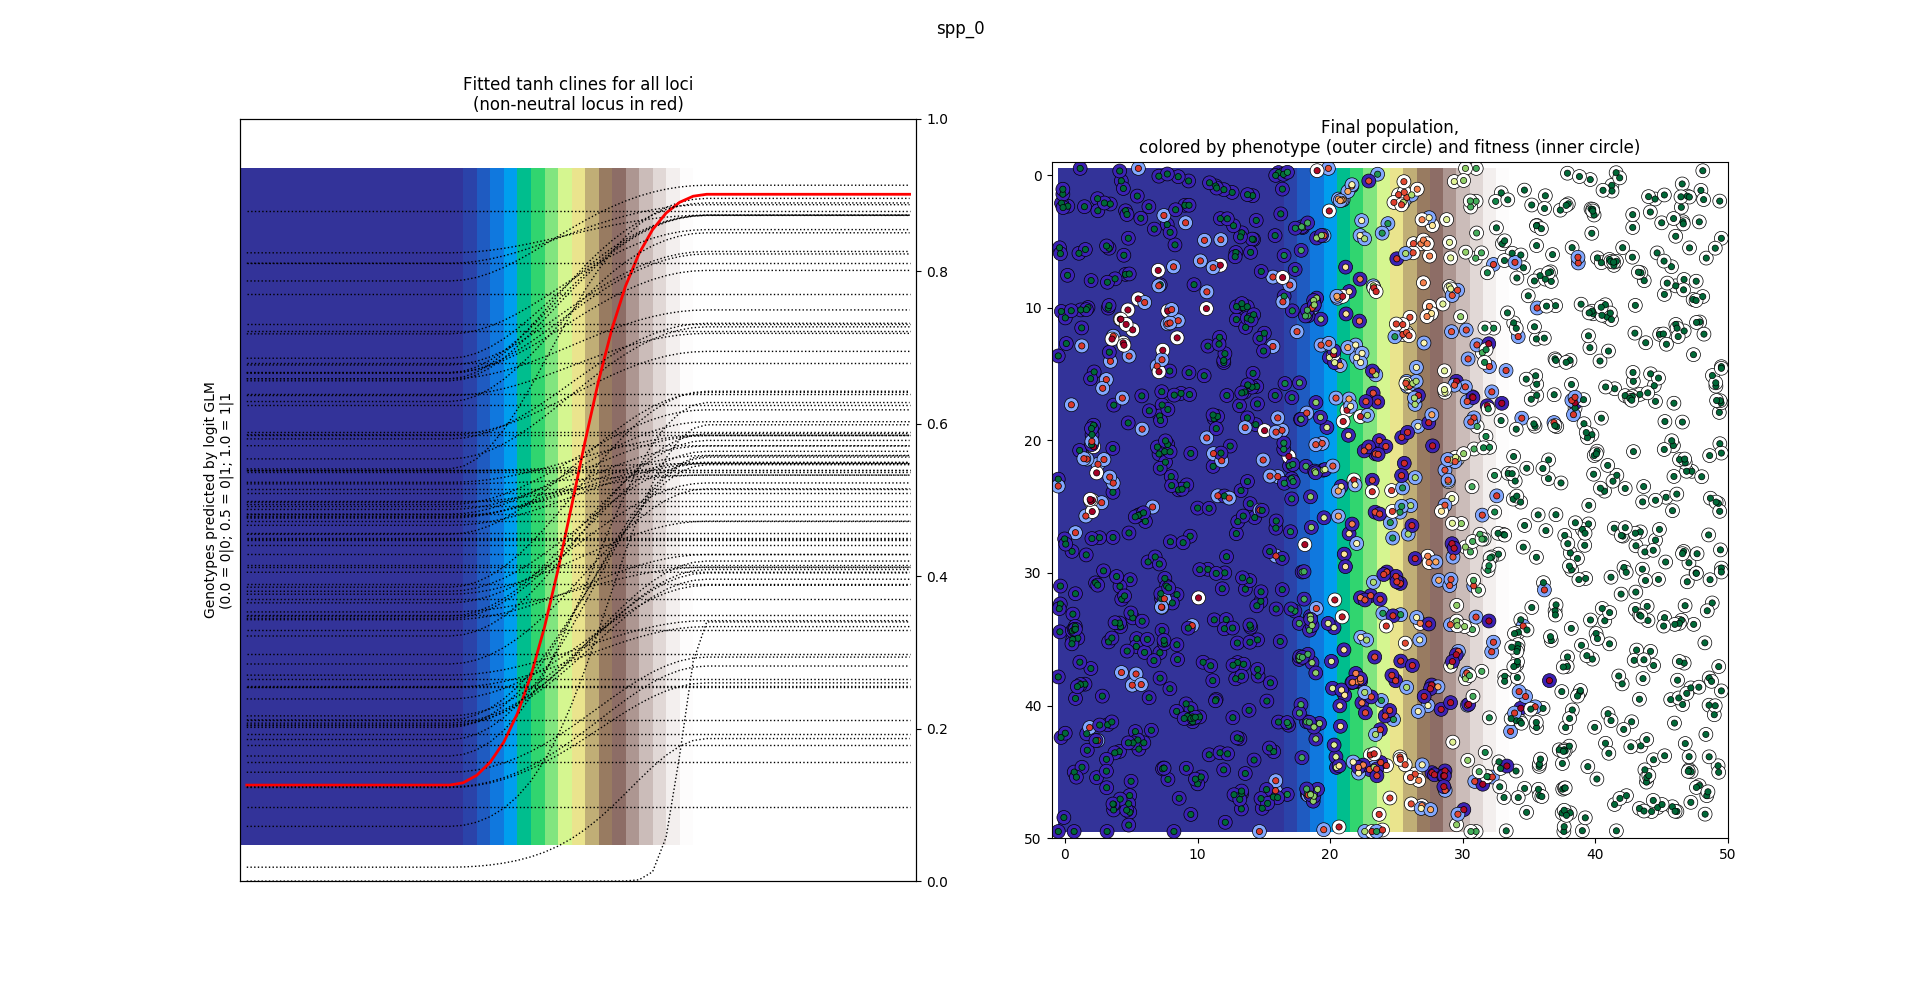
\includegraphics[width=175mm]{./img/validation/cline/cline_adaptation_phi_0pt01_2500_timesteps.png}
        \caption{Cline test: left: plot of allele-frequency clines (neutral loci in black, selective locus in bold red) against the selective landscape layer (horizontal gradient from blue to white); right: map of the final population on top of the selective lanscape layer, with individuals colored by phenotype (out circles) and fitness (inner circles)}
        \label{fig:cline}
\end{figure}


% fig 12
\begin{figure}[h!]
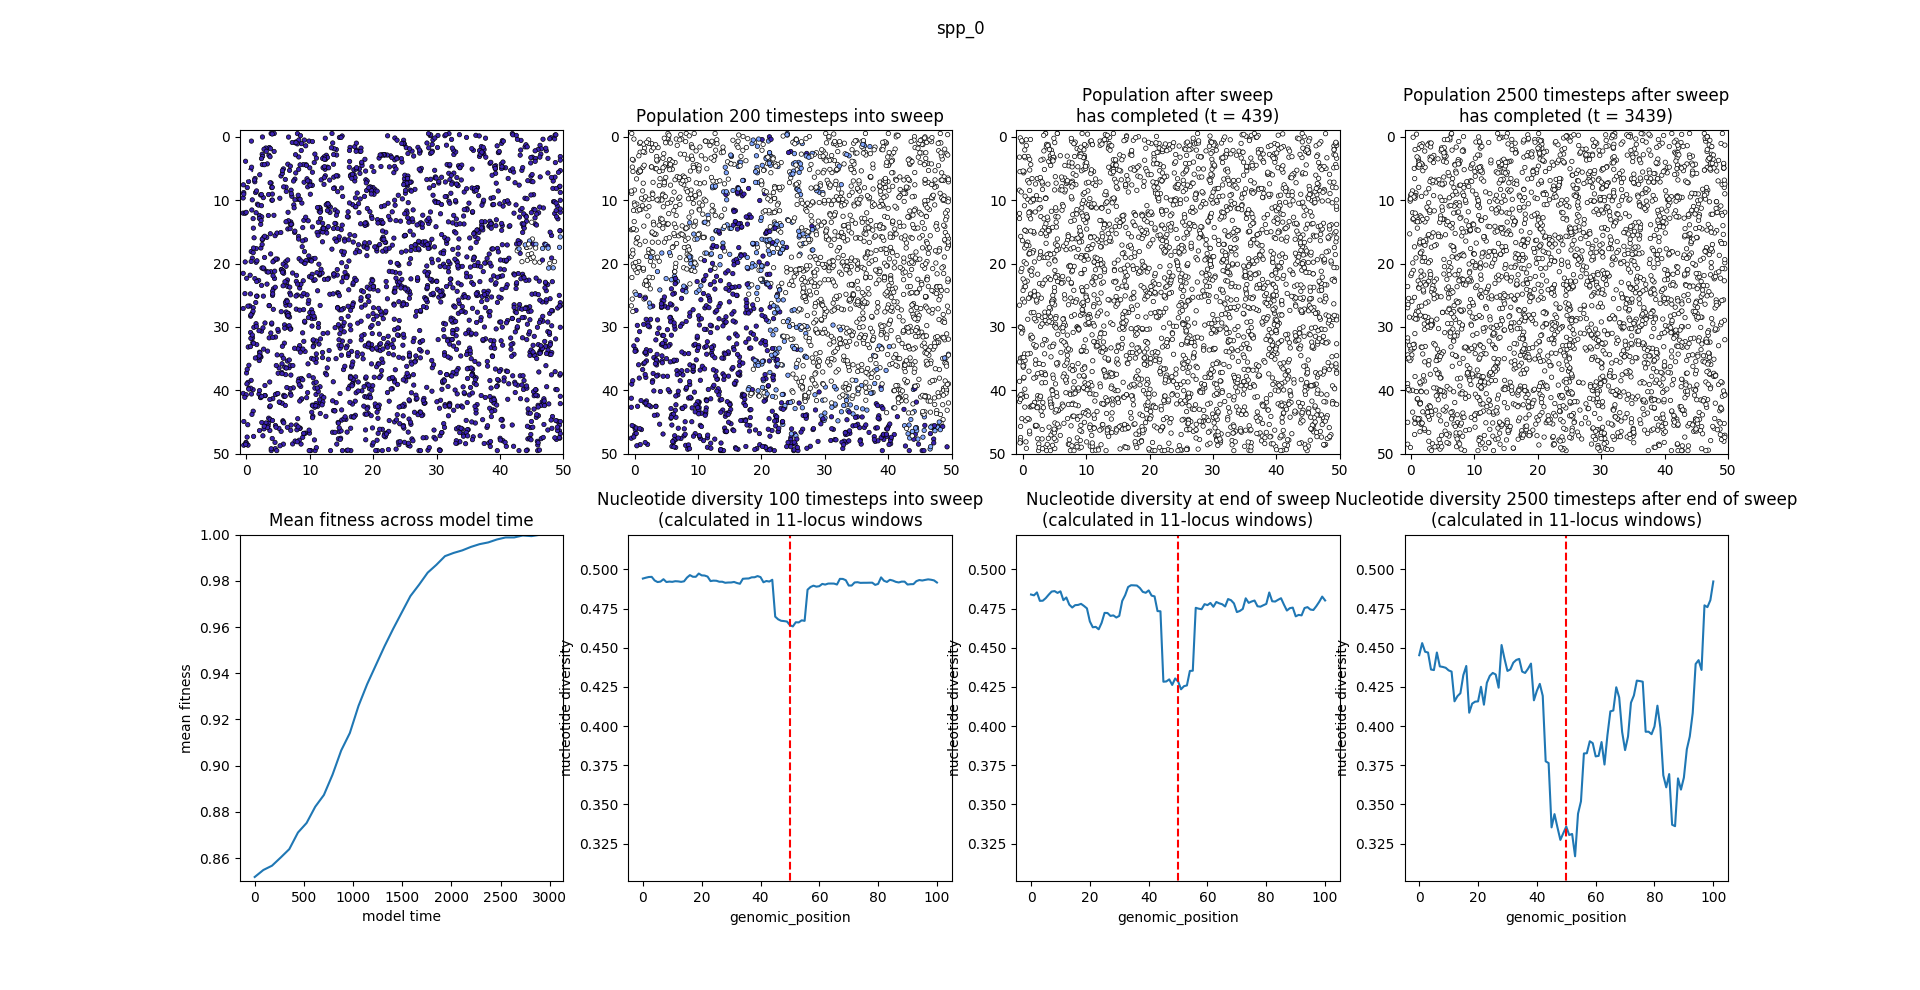
\includegraphics[width=175mm]{./img/validation/sweep/sweep_results.png}
        \caption{Selective sweep test: top row: Maps of population (colored by phenotype) at various points in model time (from left to right: timestep 0, timestep 200, after completion of sweep, and 2500 timesteps after completion of sweep); bottom row: mean fitness as a function of model time (first plot on left) and genome-wide nucleotide diversity at timestep 200, immediately after completion of sweep, and 2500 timesteps after completion of sweep (second, third, and fourth plots from left)}
        \label{fig:sweep}
\end{figure}


% fig 13
\begin{figure}[h!]
        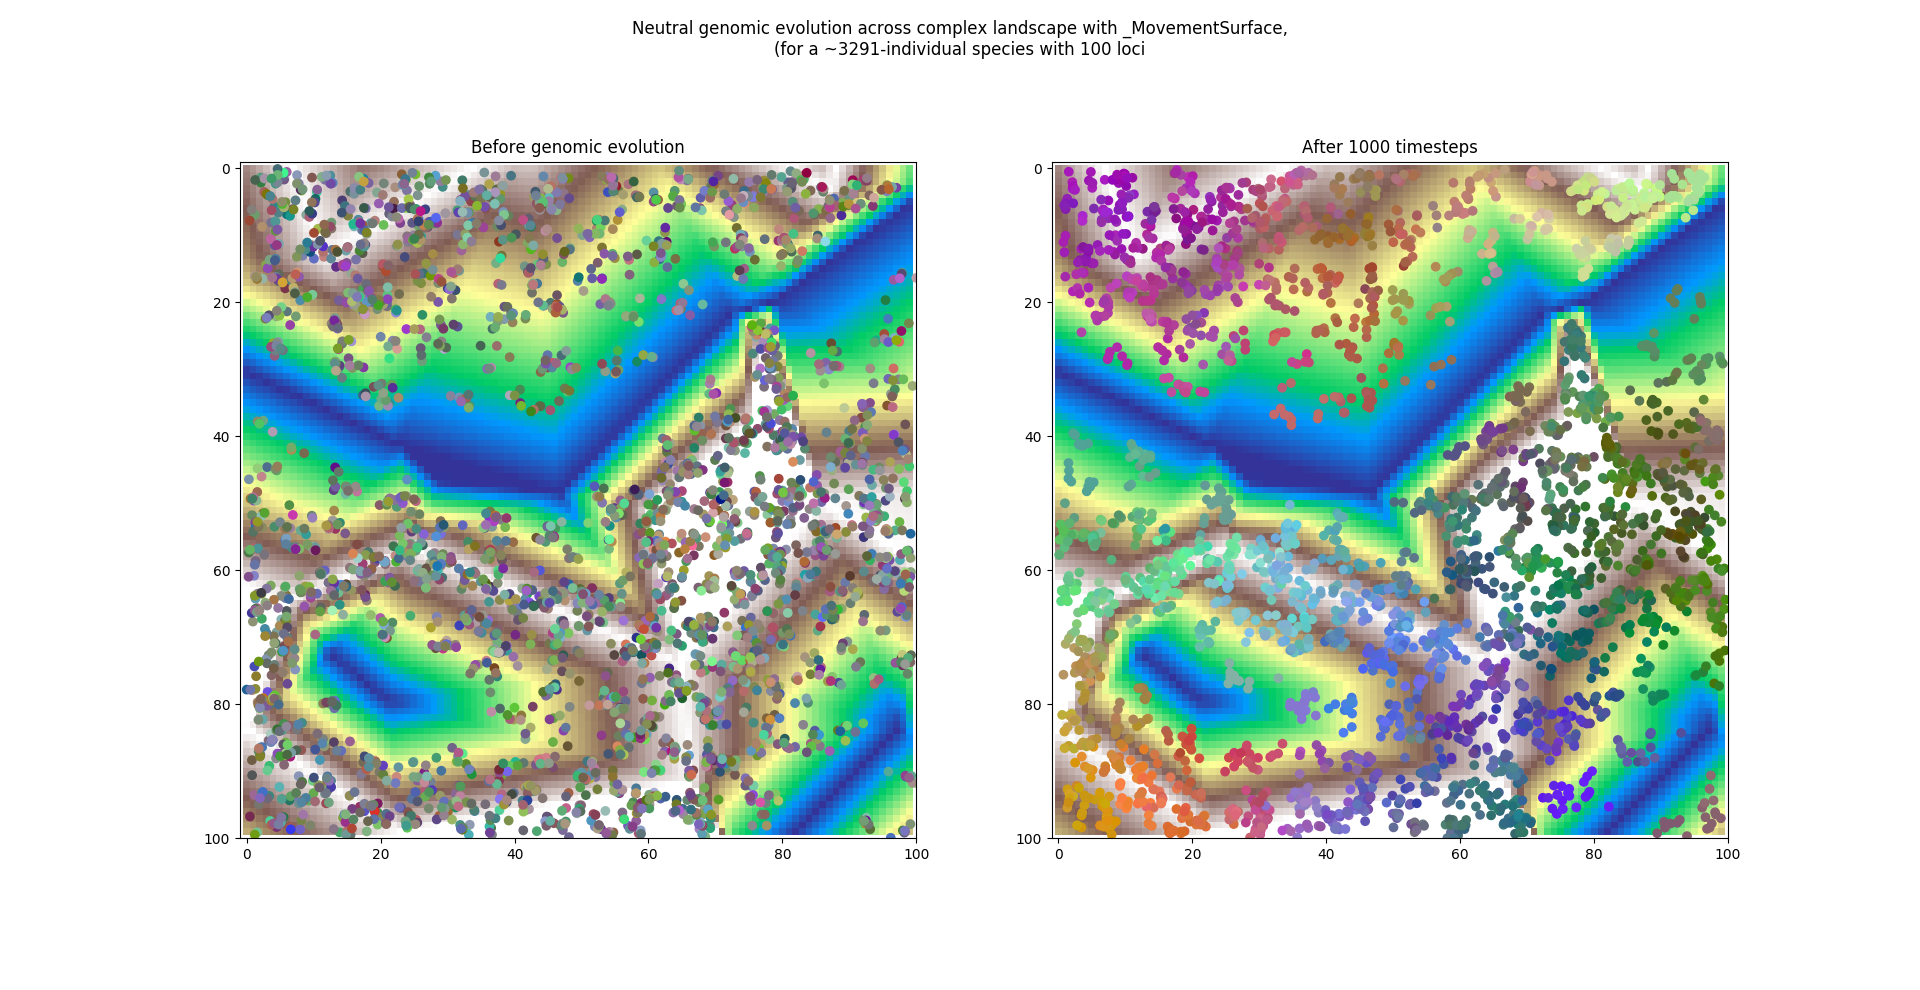
\includegraphics[width=175mm]{./img/validation/PCA/PCA_plot.png}
        \caption{Spatial structure in a species evolving on a complex landscape layer serving as a movement surface, before (left) and after (right) 1000 timesteps of neutral evolution. Individuals' colors are derived from their values for the first three PCs of a genetic PCA (each PC scaled to $0\leq value\leq$, then used to assign RGB values)}
        \label{fig:PCA}
\end{figure}


% fig 14
\begin{figure}[h!]
        \includegraphics[width=175mm]{./img/validation/two-trait/two-trait_plot.png}
        \caption{Results of simultaneous selection on two traits with divergent maps of selective force. Each trait has 10 unlinked loci and a selection coefficient of $\phi = 0.05$}
        \label{fig:two_trait_unlinked}
\end{figure}


% fig 15
\begin{figure}[h!]
        \includegraphics[width=175mm]{./img/validation/two-trait/two-trait_plot_LINKED.png}
        \caption{Results of simultaneous selection on two traits with divergent maps of selective force. Each trait has 10 linked loci (recombination rate = 0.05) and a selection coefficient of $\phi = 0.05$}
        \label{fig:two_trait_linked}
\end{figure}


% fig 16
\begin{figure}[h!]
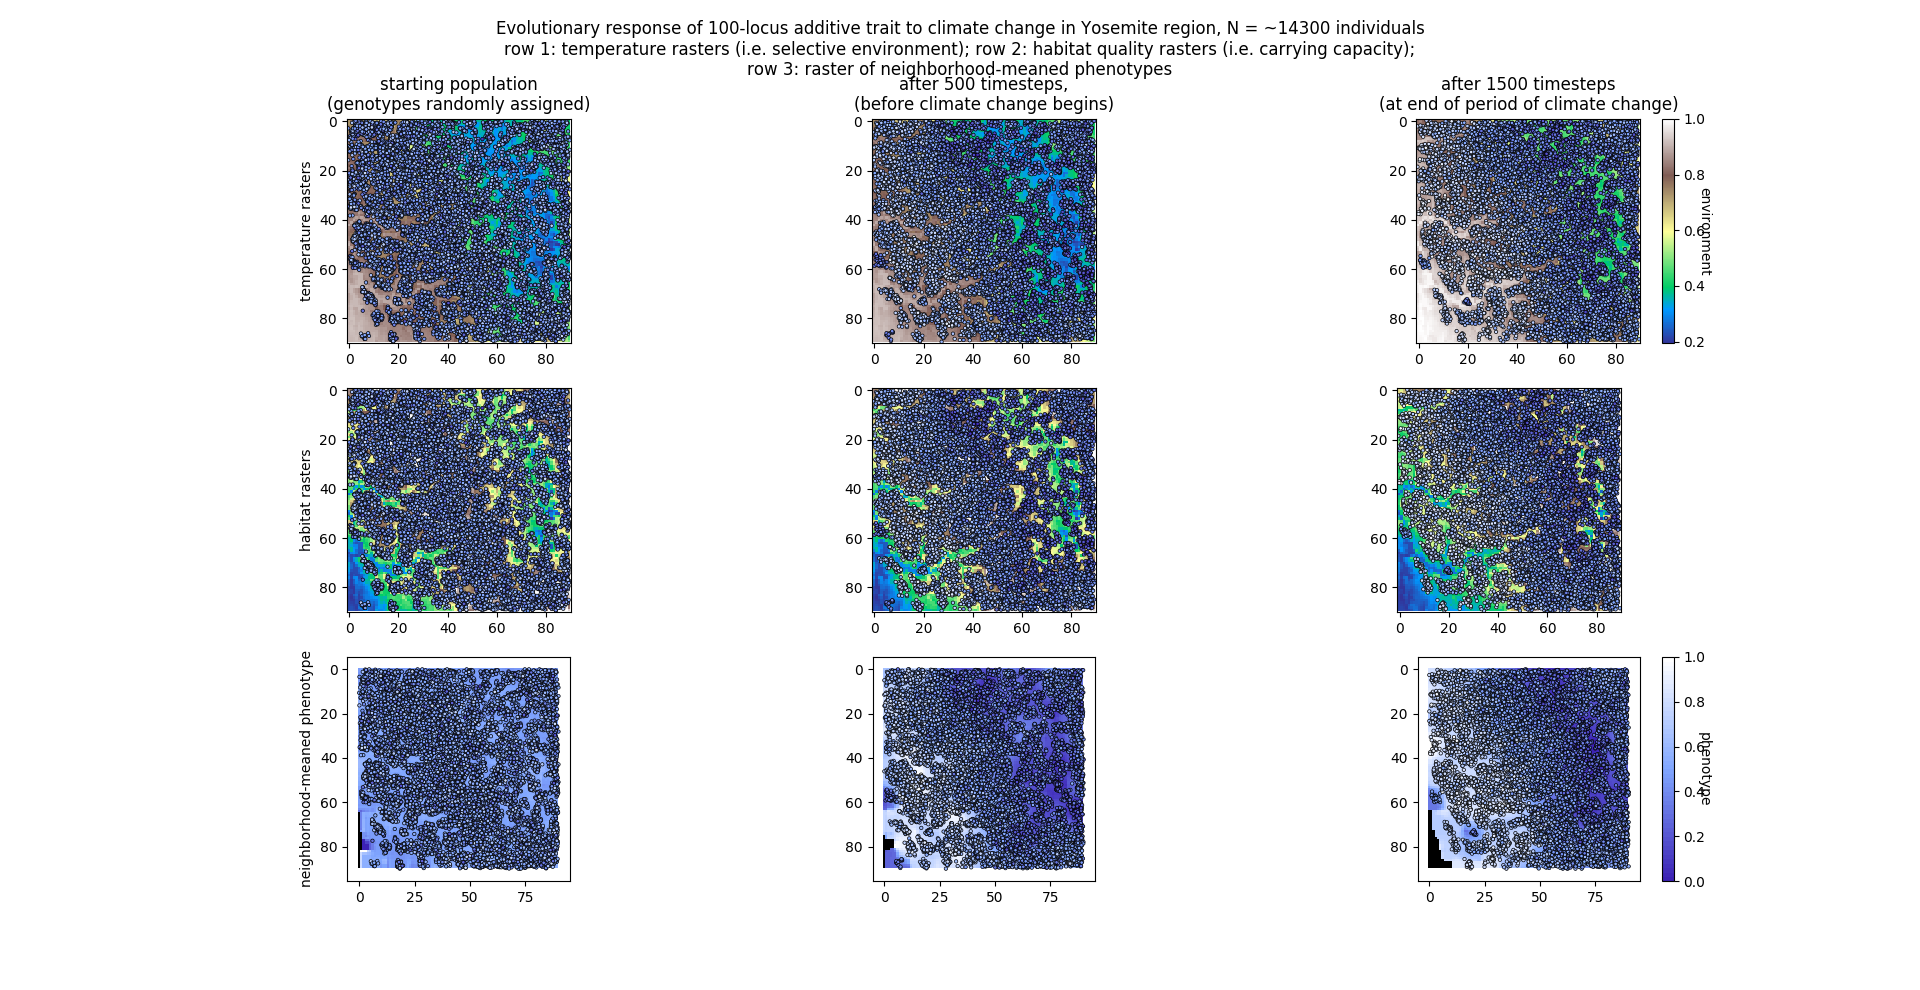
\includegraphics[width=175mm]{./img/example/yosemite_results.png}
        \caption{Temperature rasters (top row), habitat rasters (middle row), rasters of neighborhood-meaned phenotype (bottom row) at timesteps 0 (left column), 500 (before beginning of climate change; center column), and 1500 (after climate change; right column) for a species with a 100-gene trait adapted to temperature}
        \label{fig:yosemite}
\end{figure}


\end{document}
